\documentclass{beamer}
\definecolor{envy}{HTML}{1A936F}
\definecolor{berry}{HTML}{C6878F}
\definecolor{turq}{HTML}{077187}
\definecolor{pgreen}{HTML}{CBE896}
\definecolor{db}{HTML}{074F57}
\colorlet{ldb}{db!55!white}
\colorlet{lpgreen}{pgreen!55!white}

\newcommand{\light}[1]{\textcolor{db!50!white}{#1}}
% New colours!
% \setbeamercolor{background canvas}{bg=GreyWhite}

\setbeamercolor{title}{fg=db, bg=pgreen!55!white}
\setbeamercolor{frametitle}{fg=db, bg=pgreen!55!white}
\setbeamercolor{normal text}{fg=db}
\setbeamercolor{block title}{fg=db,bg=pgreen!55!white}
%%\setbeamercolor{title}{fg=black, bg=pgreen!55!white}
%%\setbeamercolor{frametitle}{fg=black, bg=pgreen!55!white}
%%\setbeamercolor{normal text}{fg=black}
%%\setbeamercolor{block title}{fg=black,bg=pgreen!55!white}
%%\setbeamercolor{block body}{fg=black!22!white}
%\setbeamercolor{alerted text}{fg=Pinky}
\setbeamercolor{itemize item}{fg=turq}
\setbeamercolor{itemize subitem}{fg=db!85!white}
\setbeamercolor{itemize subsubitem}{fg=db!85!white}
%\setbeamercolor{framesource}{fg=Carrot}
%\setbeamercolor{section in toc}{fg=PurpNav}
\setbeamercolor{footnote}{fg=black}
\setbeamercolor{footnote mark}{fg=black}
\setbeamercolor{myfootlinetext}{fg=black}
\setbeamertemplate{itemize subitem}{fg=turq}
\setbeamertemplate{itemize subsubitem}{fg=turq}
%\setbeamertemplate{itemize item}{\color{DarkPurple}$\blacksquare$}
%\setbeamertemplate{itemize item}{\color{DarkPurple}}[circle]
\setbeamertemplate{itemize item}[circle]

\newcommand{\be}{\begin{enumerate}}
	\newcommand{\ee}{\end{enumerate}}
\newcommand{\bi}{\begin{itemize}}
	\newcommand{\ei}{\end{itemize}}
\newcommand{\ccbb}{\cellcolor{turq!15!white}}
\newcommand{\cc}{\cellcolor{pgreen!55!white}}
\newcommand{\ccb}{\cellcolor{berry!35!white}}

% source at bottom left of slide
\newcommand{\sourceleft}[1]{\begin{textblock*}{4cm}(0.3cm,8.8cm)
		\begin{beamercolorbox}[ht=0.5cm,left]{framesource}
			\usebeamerfont{framesource}\usebeamercolor[fg]{framesource}
			{#1}
		\end{beamercolorbox}
	\end{textblock*}}
	
% source at bottom right of slide
\newcommand{\sourceright}[1]{\begin{textblock*}{}
		\begin{beamercolorbox}[ht=0.5cm,left]{framesource}
			\usebeamerfont{framesource}\usebeamercolor[berry]{framesource}
			{#1}
		\end{beamercolorbox}
	\end{textblock*}}

\newcommand{\cfcite}[1]{\footnote{\citeauthor{#1}, \citeyear{#1}}}

\newcommand{\sourceextremeright}[1]{\begin{textblock*}{4cm}(10.6cm,8.8cm)
		\begin{beamercolorbox}[ht=0.5cm,left]{framesource}
			\usebeamerfont{framesource}\usebeamercolor[fg]{framesource}
			{#1}
		\end{beamercolorbox}
	\end{textblock*}}

\usetheme{boxes}
\usepackage[absolute,overlay]{textpos}
%\usecolortheme{beaver}
\useinnertheme{circles}
\usepackage{amsmath}
\usepackage{amssymb}
\usepackage{lmodern}
\usepackage{xcolor}
\usepackage{tikz-cd}
\usepackage{tikz}
\usepackage{beamerthemesplit} %for the pause on the quad slide?
\usetikzlibrary{arrows.meta}
\usetikzlibrary{decorations.markings}
\usetikzlibrary{calc, arrows}
\usepackage{longtable}
\usepackage{graphicx}% http://ctan.org/pkg/graphicx
\usepackage{booktabs}
\usepackage{xspace}
\usepackage{varwidth}
\usepackage{array} %make columns all same width
%\newcolumntype{C}{>{\centering\arraybackslash}p{0.2\linewidth}}
%\usepackage{scrtime} % for \thistime (this package MUST be listed first!)
\usepackage{amsmath} % essential for cases environment
\usepackage{amsthm} % for theorems and proofs
\usepackage{amsfonts} % mathbb
\usepackage{graphics,graphicx}
\usepackage{multirow} % fancy tables
\usepackage{wasysym} % circle symbols (including half-filled circles)
\usepackage{enumerate} % fancier enumeration (e.g., a,b,c, ...)
%\usepackage{xcolor}
\usepackage{color}
\usepackage{xstring}
\usepackage[linguistics]{forest}
\usetikzlibrary{calc, arrows}
\usepackage{xcolor,colortbl}
\usepackage[export]{adjustbox}
\usepackage{array} %to uncover one col at a time of a table
%\colorlet{grey}{black!10}
%below adds slide number without putting total number of slides
\setbeamertemplate{footline}{%
	\raisebox{8pt}{\makebox[\paperwidth]{\hfill\makebox[10pt]{\scriptsize\insertframenumber}}}}

\newenvironment{itmenv}{\only{\setbeamercolor{local structure}{fg=gray}}}{}
\setbeamertemplate{enumerate items}[default]
\setbeamercolor*{enumerate item}{fg=db}

\setbeamercolor*{enumerate subitem}{fg=db}

\newcommand\FrameText[1]{%
	\begin{textblock*}{\paperwidth}(0pt,\textheight)
		\raggedleft #1\hspace{4em}\vspace{20em}
	\end{textblock*}}

\mode<presentation>
\title{\Huge Clever title here}

\author[Daniella Lato]{\\ \textbf{Daniella Lato and Jana Taha}\\ Stats 744: Final Project\\ December 3, 2019}
\date[2017]{}
\IfFileExists{upquote.sty}{\usepackage{upquote}}{}
\newcommand{\itm}{\item<itm@1->}
\newcommand{\btVFill}{\vskip0pt plus 1filll}
\newcommand{\s}{\textit{Sinorhizobium}\ }
\newcommand{\sm}{\textit{Sinorhizobium meliloti}\xspace}
\newcommand{\salm}{\textit{Salmonella enterica}\xspace}
\newcommand{\smel}{\textit{S.\,meliloti}\xspace}
\newcommand{\smed}{\textit{S.\,medicae}}
\newcommand{\sfred}{\textit{S.\,fredii}}
\newcommand{\ssah}{\textit{S.\,saheli}}
\newcommand{\ster}{\textit{S.\,terangae}}
\newcommand{\ag}{\textit{Agrobacterium tumefaciens }}
\newcommand{\p}{progressiveMauve\xspace}
\newcommand{\agro}{\textit{A.\,tumefaciens }}
\newcommand{\bur}{\textit{Burkholderia}\xspace}
\newcommand{\vib}{\textit{Vibrio}\xspace}
\newcommand{\bor}{\textit{Bordetella}\xspace}
\newcommand{\xan}{\textit{Xanthomonas}\xspace}
\newcommand{\sul}{\textit{Sulfolobus}\xspace}
\newcommand{\ent}{\textit{Enterobacteria}\xspace}
\newcommand{\bac}{\textit{Bacillus subtilis}\xspace}
\newcommand{\ecoli}{\textit{Escherichia coli}\xspace}
\newcommand{\lis}{\textit{Listeria monocytogenes}\xspace}
\newcommand{\bass}{\textit{B.\,subtilis}\xspace}
\newcommand{\bas}{\textit{Bacillus subtilis}\xspace}
\newcommand{\tub}{\textit{Mycobacterium tuberculosis}\xspace}
\newcommand{\strep}{\textit{Streptomyces}\xspace}
\newcommand{\agrot}{\textit{Agrobacterium tumefaciens}\xspace}
\newcommand{\ecol}{\textit{E.\,coli}\xspace}
\newcommand{\salb}{\textit{S.\,alblus}\xspace}
\newcommand{\salbus}{\textit{S.\,albus}\xspace}
\newcommand{\shyg}{\textit{S.\,hygroscopicus}\xspace}
\newcommand{\sliv}{\textit{S.\,lividans}\xspace}
\newcommand{\sros}{\textit{S.\,roseosporus}\xspace}
\newcommand{\ssir}{\textit{S.\,sirex}\xspace}
\newcommand{\sven}{\textit{S.\,venezuelae}\xspace}
\newcommand{\scoe}{\textit{S.\,coelicolor}\xspace}
\newcommand{\hal}{\textit{Haloquadratum walsbyi}\xspace}
\newcommand{\pa}{pSymA\xspace}
\newcommand{\pb}{pSymB\xspace}
\newcommand{\ch}{$\checkmark$}
\setbeamertemplate{navigation symbols}{}
\newcommand*{\NodeSize}{0.5cm}%
\newcommand*{\YShiftBetweenRows}{-1cm}% Subsequent rows are shited down so they don't overlap
%\tikzset{DNA Style/.style={minimum size=0.5cm, draw=gray, line width=1pt}}{}
\providecommand{\e}[1]{\ensuremath{\times 10^{#1}}}
\newlength{\YShift}% 
\newcounter{ColumnCounter}% Prefix for node labels

\newcommand\FourQuad[4]{%
	\begin{minipage}[b][.35\textheight][t]{.47\textwidth}#1\end{minipage}\hfill%
	\begin{minipage}[b][.35\textheight][t]{.47\textwidth}#2\end{minipage}\\[0.5em]
	\begin{minipage}[b][.35\textheight][t]{.47\textwidth}#3\end{minipage}\hfill
	\begin{minipage}[b][.35\textheight][t]{.47\textwidth}#4\end{minipage}%
}

% Initialize - These are probably not needed, but prefer to set them
\setlength{\YShift}{0cm}% 
\setcounter{ColumnCounter}{0}


%%%%%%%%%%%%%%%%%%%%%%%%%%%%%%%%%%%%%%%%%%%%%%%%%%%%%%%%%%%%%%%%%%%%%%%%%%%%%%%%%%%%%%%%%%%%%%%%%%%%%%%%%%%%%%%%%%%%%%%%%%%%%%%%%%%%%%%%%%%%%%%%%%%%%%%%%%%%%%%%


\begin{document}
% \titlegraphic{text} %for including logos in title. have to adjust vspace and hspace	
	\begin{frame}
		
		\titlepage
		
	\end{frame}
	%\begin{frame}
	%\begin{center}
	
	%\huge{Introduction}
	
	%\end{center}
	%\end{frame}
%%%%%%%%%%%%%%%%%%%%%%%%%%%%%%%%%%%%%%%%%%%%%%%%%%%%%%%
\begin{frame}{The Organism}
	\begin{columns}[t]
	\column{0.5\textwidth}	
	Bacteria:
	\bi
	\itm \ecoli
	\itm \bas
	\itm \strep
	\itm \sm
	\ei
	\column{0.5\textwidth}
	\textbf{insert pic of bacteria here! probs sino bc its beautiful}
	\end{columns}
\end{frame}
%%%%%%%%%%%%%%%%%%%%%%%%%%%%%%%%%%%%%%%%%%%%%%%%%%%%
\begin{frame}[t]{Biological Background}
	\bigskip
	\begin{columns}[t]
		\column{0.30\textwidth}
		\textbf{1) Circular}
		\centering
		\begin{tikzpicture}
		%circle
		\draw[thick] (4,0) circle (1cm);
		%origin tick
		\draw[thick] (4,0.8) -- (4,1.2);
		\tikzstyle{none}=[draw = none, minimum width=2cm, minimum height=0.3cm, rounded corners]
		\node[none] (first reservoir) at (4,-4) {\ecoli};
		\tikzstyle{ntwo}=[draw = none, minimum width=2cm, minimum height=0.3cm, rounded corners]
		\node[ntwo] (second reservoir) at (4,-4.5) {\bas};
		\end{tikzpicture}
		
		\column{0.30\textwidth}
		\textbf{2) Linear}
		\centering
		
		\bigskip
		\begin{tikzpicture}
	%line
		\draw[thick] (3.5,0) -- (6.5,0);
		%origin tick
		\draw[thick] (4.5,-.2) -- (4.5,.2);
		\tikzstyle{none}=[draw = none, minimum width=2cm, minimum height=0.3cm, rounded corners]
		\node[none] (first reservoir) at (5,-5.1) {\strep};
		\end{tikzpicture}
		
		\column{0.4\textwidth}
		\textbf{3) Multi-repliconic}
		\centering
		\begin{tikzpicture}
		%chrom
		\draw[thick] (0,0) circle (1cm) node {\tiny Chromosome};
		%ori tick
		\draw[thick] (0,0.8) -- (0,1.2);
		%pSymA
		\draw[thick] (0,-1.75) circle (0.5cm) node {\tiny \pa};
	%ori tick
		\draw[thick] (0,-1.1) -- (0,-1.4);
		%pSymB
		\draw[thick] (0,-3.25) circle (0.75cm) node {\tiny \pb};
		%ori tick
		\draw[thick] (0,-2.35) -- (0,-2.65);
		\tikzstyle{none}=[draw = none, minimum width=2cm, minimum height=0.3cm, rounded corners]
		\node[none] (first reservoir) at (0,-4.5) {\sm};
		\end{tikzpicture}
	\end{columns}
\end{frame}
%%%%%%%%%%%%%%%%%%%%%%%%%%%%%%%%%%%%%%%%%%%%%%%%%%%
%%%%%%%%%%%%%%%%%%%%%%%%%%%%%%%%%%%%%%%%%%%%%%%%%%%%
\begin{frame}[t]{Bacterial Genome Properties}
	\begin{columns}[t]
		\begin{column}{0.5\textwidth}
	Bidirectional Replication
		\bi
		\itm Gene dosage
		\itm Sequence composition
		\itm Codon bias
		\itm Replication errors
		\itm Strand differences
		\ei
	\bigskip
	
		\centering{
			\resizebox{\textwidth}{!}{%
				\begin{tikzpicture}
			
	%new DNA label
	\node[berry] at (0.15,-2) {\fontsize{1}{1}\selectfont \textbf{-- new DNA}};
	%old DNA label
	\node[] at (0.15,-2.05) {\fontsize{1}{1}\selectfont \textbf{-- old DNA}};
				\end{tikzpicture}
			}%resiebox
		}%centering
\end{column}
\begin{column}{0.5\textwidth}
%	\centering{
%		\resizebox{\textwidth}{!}{%
%			\begin{tikzpicture}
%			%fig lable A
%			\node[berry] at (0,0) {\fontsize{10}{3}\selectfont \textbf{-- new DNA}};
%			\end{tikzpicture}
%		}%resiebox
%	}%centering
		\centering{
			\resizebox{\textwidth}{!}{%
				\begin{tikzpicture}[x=0.5cm, y=0.5cm]
				\tikzstyle{neleven}=[draw = none, minimum width=0.05cm, minimum height=0.05cm, berry]
				%new DNA label
%				\node[neleven] at (0.15,-3) {\fontsize{1}{1}\selectfont \textbf{-- new DNA}};
%				\draw[line width=0.01mm,
%				postaction={decorate}, fill=black] (0,-2.5) circle (0.008cm);
%				\draw[line width=0.01mm,
%				postaction={decorate}, fill=pink] (0.15,-2.9) circle (0.008cm);
				%%% TOP CIRCLE %%%
				%rep bubble circle
%				\draw[line width=0.01mm,
%				postaction={decorate}] (0,-2.3) ellipse (0.05cm and 0.02cm);
				%old DNA outter circle
				\draw[line width=0.05mm,
				postaction={decorate}] (0,-2.5) circle (0.1cm);
				%old DNA top arc
				\draw[line width=0.05mm] (0.153,-2.4) arc (-80:-100:0.44cm);
				%old DNA bottom arc
				\draw[line width=0.05mm] (0.15,-2.4) arc (30:-210:0.086cm);
				%new DNA top arc
				\draw[line width=0.05mm, berry] (0.136,-2.383) arc (40:140:0.09cm);
				%new DNA bottom arc
				\draw[line width=0.05mm, berry] (0.136,-2.38) arc (-80:-100:0.394cm);
				%old DNA inner circle
%				\draw[line width=0.01mm,
%				postaction={decorate}] (0,-2.5) circle (0.09cm);
				%arrow inbtwn circles
				\draw[-{Latex[width=0.1mm,length=0.2mm]},line width = 0.03mm] (0,-2.72) -- (0,-2.79);
				%%% BOTTOM CIRCLE %%%
				%old DNA outter circle
				\draw[line width=0.05mm,
				postaction={decorate}] (0,-3) circle (0.1cm);
%				%old DNA inner circle
%				\draw[line width=0.01mm,
%				postaction={decorate}] (0,-3) circle (0.09cm);
				%old DNA bottom arc
				\draw[line width=0.05mm] (0.15,-2.9) arc (0:-180:0.0748cm);
				%old DNA Inner arc
				\draw[line width=0.05mm] (0.15,-2.9) arc (30:-210:0.086cm);
				%new DNA top arc
				\draw[line width=0.05mm, berry] (0.1369,-2.882) arc (40:140:0.089cm);
				%new DNA bottom arc
				\draw[line width=0.05mm, berry] (0.1369,-2.881) arc (0:-180:0.068cm);
				%arrow for rep to the right
				\draw[-{Latex[width=0.1mm,length=0.2mm]},line width = 0.03mm] (0.05,-2.881) -- (0.13,-2.881);
				%arrow for rep to the left
				\draw[-{Latex[width=0.1mm,length=0.2mm]},line width = 0.03mm] (-0.05,-2.881) -- (-0.13,-2.881);

				\end{tikzpicture}
			}%resiebox
		}%centering


	\end{column}
\end{columns}
	\btVFill
		\tiny \vspace{-\baselineskip}\color{berry}{Rocha 2004, Quax et al. 2015, Hyrien et al. 2013}
\end{frame}

%%%%%%%%%%%%%%%%%%%%%%%%%%%%%%%%%%%%%%%%%%%%%%%%%%%
%%%%%%%%%%%%%%%%%%%%%%%%%%%%%%%%%%%%%%%%%%%%%%%%%%%%%%%
\begin{frame}{Bacterial Genomes}
\Large
\centering
	Different \textbf{replicons} and \textbf{positions} of bacterial genomes can have \textbf{varying molecular trends}
	
	
\end{frame}

%%%%%%%%%%%%%%%%%%%%%%%%%%%%%%%%%%%%%%%%%%%%%%%%%%%%

\begin{frame}{Spatial Molecular Trends}
	\begin{columns}[t]
		\column{.5\textwidth}
		\centering
		\includegraphics[width=0.67\textwidth]{./presentation_graphs/mut_graph.pdf}\\
		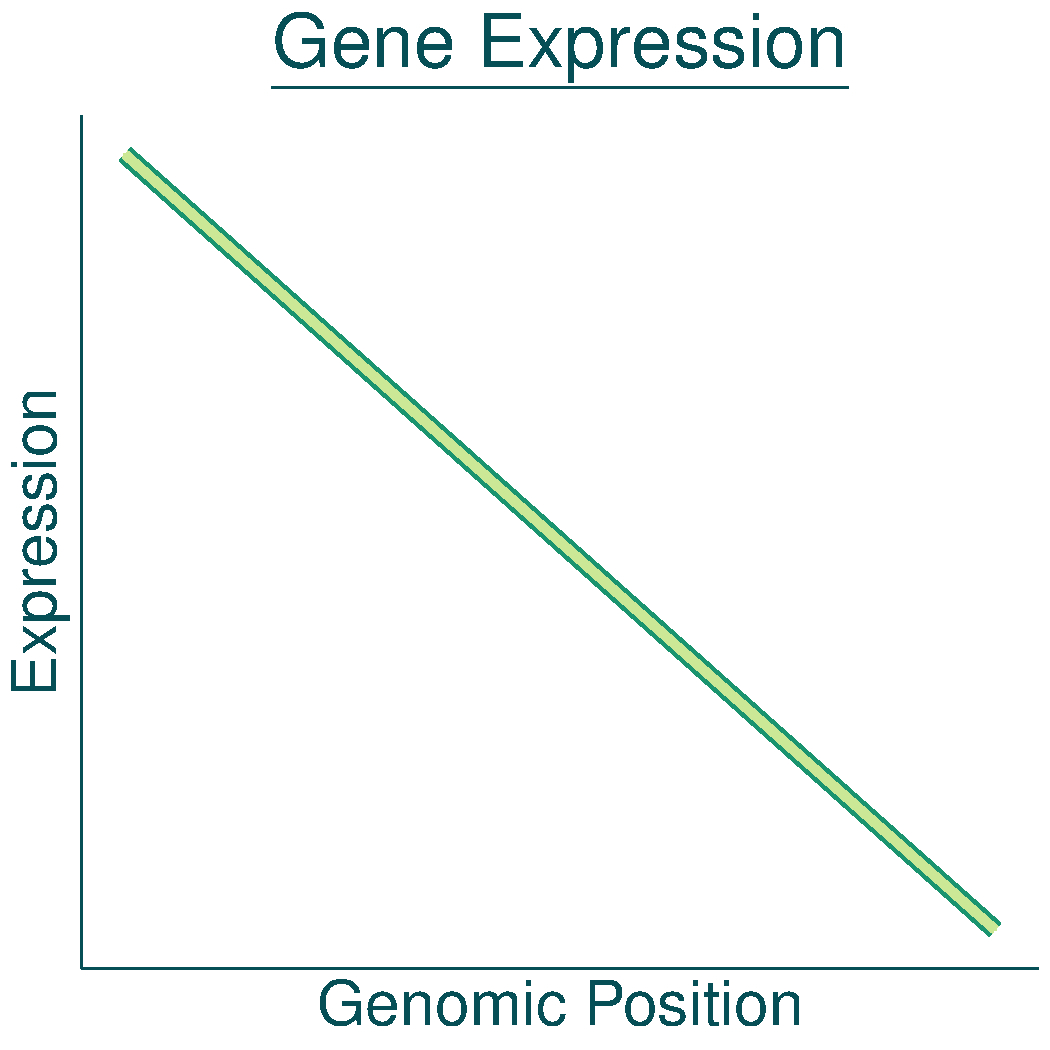
\includegraphics[width=0.67\textwidth]{./presentation_graphs/exp_graph.pdf}
		\column{.5\textwidth}
		\centering
		\includegraphics[width=0.67\textwidth]{./presentation_graphs/ess_graph.pdf}\\
		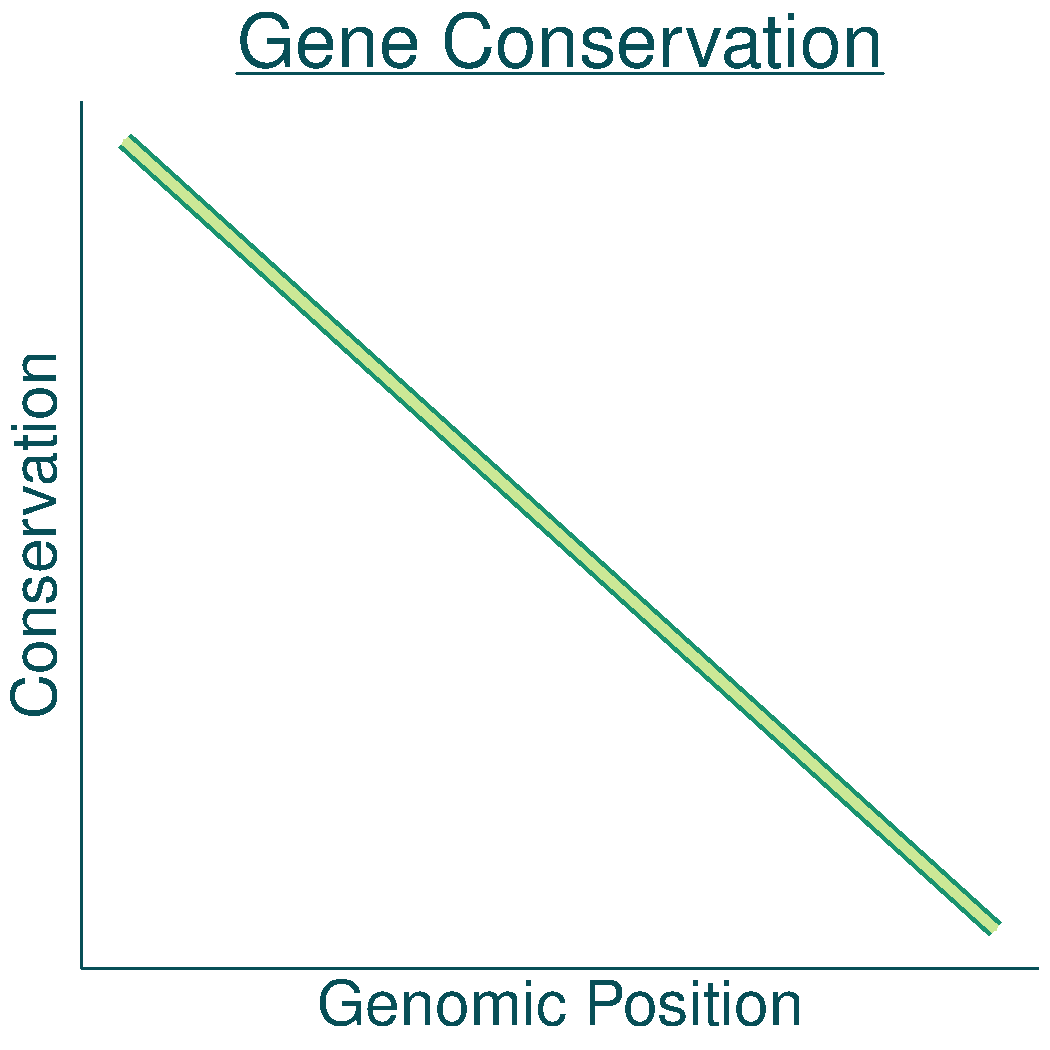
\includegraphics[width=0.67\textwidth]{./presentation_graphs/cons_graph.pdf}
	\end{columns}
	
	\btVFill
	\tiny \vspace{-\baselineskip}\color{berry}{Couturier et al. 2006, Cooper et al. 2010, Sharp et al. 2005, Morrow et al. 2012, Cooper and Rocha 2006}
	%		\sourceright{Couturier et al. 2006, Cooper et al. 2010, Sharp et al. 2005, Morrow et al. 2012, Cooper and Rocha 2006}
	
\end{frame}
%%%%%%%%%%%%%%%%%%%%%%%%%%%%%%%%%%%%%%%%%%%%%%%%%%%%%%%
\begin{frame}{Selection}
	Measuring what evolutionary forces are acting on genes
	\bi
	\itm \textbf{dN} = non-synonymous substitution rate
		\bi
		\itm change in amino acid sequence
		\itm can alter function of the protein
		\ei
	\itm \textbf{dS} = synonymous substitution rate
		\bi
		\itm no change in amino acid sequence
		\itm will not alter function of protein
		\ei
	\itm \textbf{ $\omega$ = (dN/dS)}
		\bi
		\itm \textbf{$\omega$ $>$ 1} $\rightarrow$ positive selection
			\bi
			\itm beneficial to the organism and will likely be maintained over time
			\ei
		\itm \textbf{$\omega$ = 1} $\rightarrow$ neutral selection
			\bi
			\itm neither beneficial nor deleterious to the organism
			\ei
		\itm \textbf{$\omega$ $<$ 1} $\rightarrow$ negative selection
			\bi
			\itm deleterious to the organism and will likely not be maintained over time
			\ei
		\ei
	\ei
\end{frame}
%%%%%%%%%%%%%%%%%%%%%%%%%%%%%%%%%%%%%%%%%%%%%%%%%%%
\begin{frame}[t]{The Data}
			\textbf{Gene Expression}
			\bi
			\itm \ecol, \bass, \strep, and \smel
			\itm Gene expression + distance from the origin of replication
			\itm \textbf{Expectation:} Near the origin or replication = Higher Expression
			\ei
		
\end{frame}
%%%%%%%%%%%%%%%%%%%%%%%%%%%%%%%%%%%%%%%%%%%%%%%%%%%
\begin{frame}[t]{The Data}
			\textbf{Selection}
			\bi
			\itm \ecol, \bass, \strep, and \smel
			\itm dN, dS, and $\omega$ $+$ distance from the origin of replication
			\itm $\omega$ $>$ 1 (positive selection), $\omega$ = 1 (neutral), $\omega$ $<$ 1 (negative selection)
			\itm \textbf{Expectations:} 
			\begin{enumerate}
				\item dS $>$ dN
				\item Most genes are under neutral or negative selection
				\item Genes that are under positive selection should most likely be accessory genes
			\end{enumerate}
			\bi
			\itm Core genes are near the origin of replication
			\itm Accessory genes are usually near the terminus
			\ei
			\ei
\end{frame}
%%%%%%%%%%%%%%%%%%%%%%%%%%%%%%%%%%%%%%%%%%%%%%%%%%
\begin{frame}{Gene Expression}
	Insert gene expression graphs here!!!!!
\end{frame}
%%%%%%%%%%%%%%%%%%%%%%%%%%%%%%%%%%%%%%%%%%%%%%%%%%
%%%%%%%%%%%%%%%%%%%%%%%%%%%%%%%%%%%%%%%%%%%%%%%%%%
\begin{frame}{Selection Summary}
	\centering
	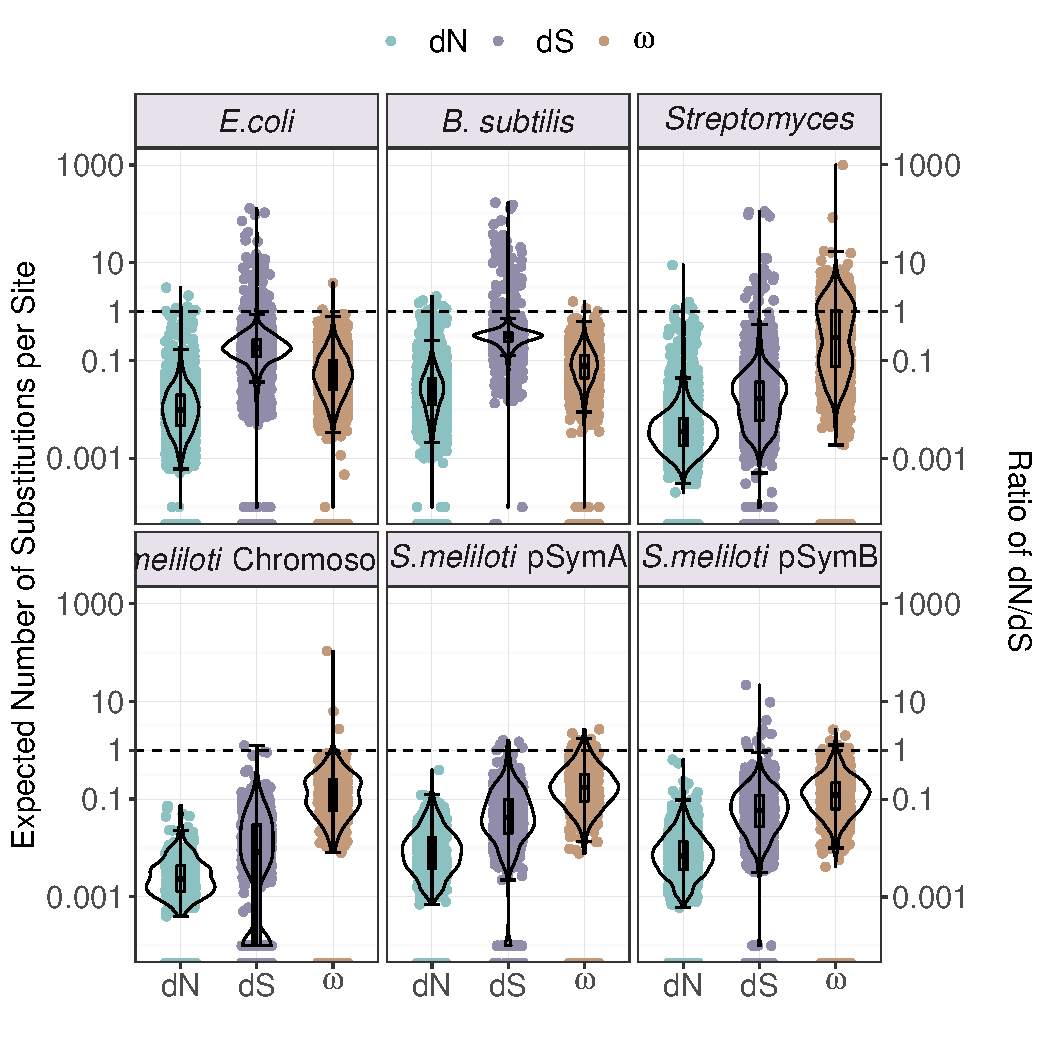
\includegraphics[width=0.8\textwidth]{selection_vio_box.pdf}
\end{frame}
%%%%%%%%%%%%%%%%%%%%%%%%%%%%%%%%%%%%%%%%%%%%%%%%%%
%%%%%%%%%%%%%%%%%%%%%%%%%%%%%%%%%%%%%%%%%%%%%%%%%%
\begin{frame}{\strep Selection}
	\centering
	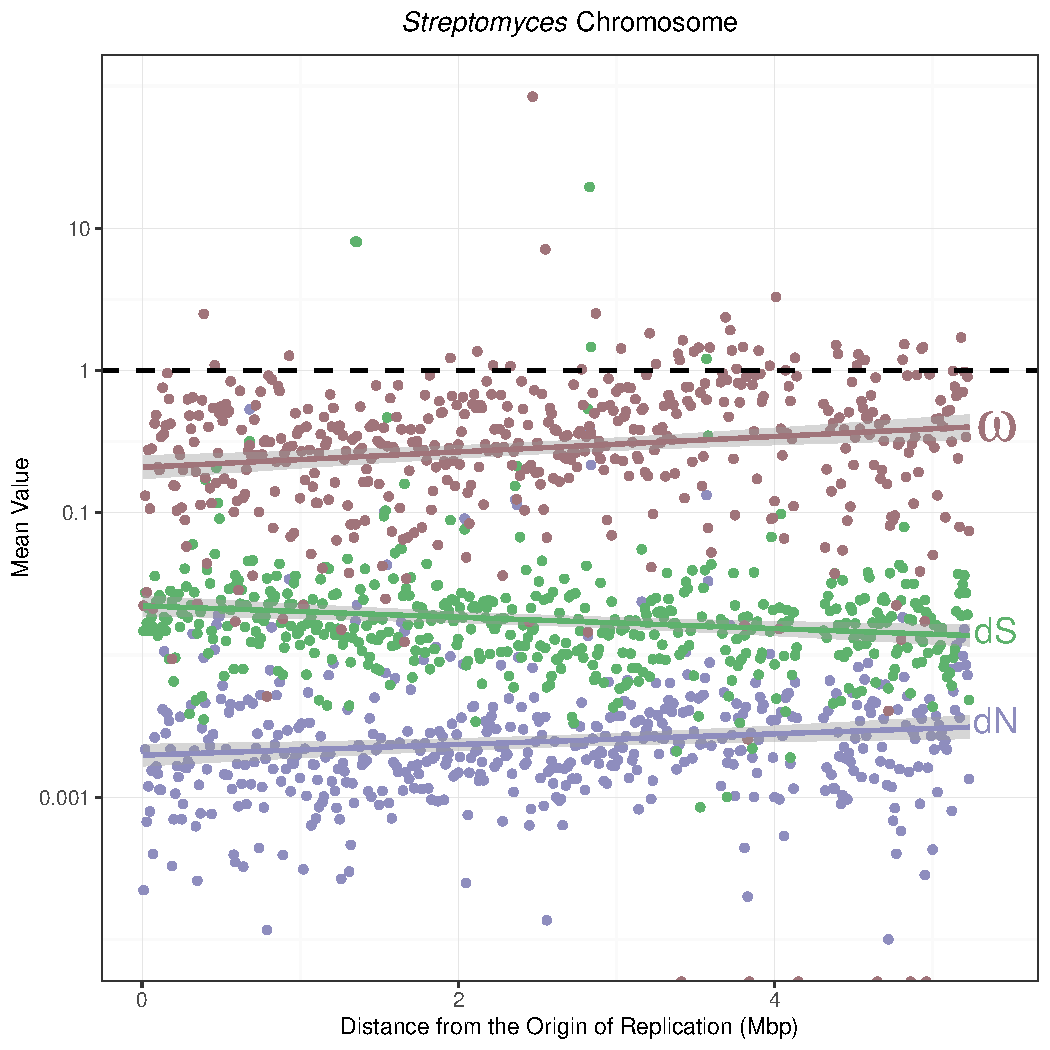
\includegraphics[width=0.77\textwidth]{strep_selection.pdf}
\end{frame}
%%%%%%%%%%%%%%%%%%%%%%%%%%%%%%%%%%%%%%%%%%%%%%%%%%

%%%%%%%%%%%%%%%%%%%%%%%%%%%%%%%%%%%%%%%%%%%%%%%%%%
\begin{frame}{Summary}
	\ch Gene expression decreases (slightly) with increasing distance from the origin of replication
	\bi
	\itm But we see more of a wave like pattern!
	\ei

	\ch dS $>$ dN

	\ch Most genes are under neutral or negative selection ($\omega$ $\le$ 1)

	\ch In \strep, genes under positive selection ($\omega$ $>$ 1) were near the terminus and most likely accessory genome
\end{frame}
%%%%%%%%%%%%%%%%%%%%%%%%%%%%%%%%%%%%%%%%%%%%%%%%%%
%\begin{frame}{}
%	\centering
%	\Huge
%	\textbf{Bacterial genomes are a mosaic of information!}
%
%\end{frame}
%%%%%%%%%%%%%%%%%%%%%%%%%%%%%%%%%%%%%%%%%%%%%%%%%%%%%%
%\begin{frame}{Bacterial Genome Reorganization}
%	\FourQuad%
%	{\centering
%		\small{\textbf{H}orizontal \textbf{G}ene \textbf{T}ransfer (\textbf{HGT})}
%		\includegraphics[angle=270, origin=c, width=0.75\textwidth]{C:/Users/Daniella/Documents/Sinorhizobium2015/Conferences/HGT_pic.pdf}}%
%	{
%	}%
%	{
%	}%
%	{ 
%		
%	}
%\end{frame}
%
%
%%%%%%%%%%%%%%%%%%%%%%%%%%%%%%%%%%%%%%%%%%%%%%%%%%%%%%
%\begin{frame}{Bacterial Genome Reorganization}
%	\FourQuad%
%	{\centering
%		\small{\textbf{H}orizontal \textbf{G}ene \textbf{T}ransfer (\textbf{HGT})}
%		\includegraphics[angle=270, origin=c, width=0.75\textwidth]{C:/Users/Daniella/Documents/Sinorhizobium2015/Conferences/HGT_pic.pdf}}%
%	{
%	}%
%	{ \centering
%		\bigskip
%		\small{Duplication}
%		\includegraphics[angle=0, origin=c, width=\textwidth]{C:/Users/Daniella/Documents/Sinorhizobium2015/Conferences/duplication_pic.pdf}
%	}%
%	{ 
%		
%	}
%\end{frame}
%
%%%%%%%%%%%%%%%%%%%%%%%%%%%%%%%%%%%%%%%%%%%%%%%%%%%%%%
%\begin{frame}{Bacterial Genome Reorganization}
%	\FourQuad%
%	{\centering
%		\small{\textbf{H}orizontal \textbf{G}ene \textbf{T}ransfer (\textbf{HGT})}
%		\includegraphics[angle=270, origin=c, width=0.75\textwidth]{C:/Users/Daniella/Documents/Sinorhizobium2015/Conferences/HGT_pic.pdf}}%
%	{\centering
%		\small{Rearrangement and Translocation}
%		\includegraphics[angle=0, origin=c, width=\textwidth]{C:/Users/Daniella/Documents/Sinorhizobium2015/Conferences/rearrangements_pic.pdf}
%	}%
%	{ \centering
%		\bigskip
%		\small{Duplication}
%		\includegraphics[angle=0, origin=c, width=\textwidth]{C:/Users/Daniella/Documents/Sinorhizobium2015/Conferences/duplication_pic.pdf}
%	}%
%	{ \centering
%		\bigskip
%		\small{Inversion}
%		\includegraphics[angle=0, origin=c, width=\textwidth]{C:/Users/Daniella/Documents/Sinorhizobium2015/Conferences/inversion_pic.pdf}
%		
%	}
%\end{frame}
%%%%%%%%%%%%%%%%%%%%%%%%%%%%%%%%%%%%%%%%%%%%%%%%%%%%%%
%\begin{frame}{Bacterial Genome Reorganization}
%	\begin{columns}[t]
%		\begin{column}{0.5\textwidth}
%			\textbf{Acquisition of genetic information in:}
%			\bi
%			\itm Resistance
%			\itm Pathogenicity
%			\itm Virulence
%			\itm Symbiosis
%			\itm Environment adaptation
%			\itm Physiology
%			\itm etc...
%			\ei
%			
%		\end{column}
%		
%%		\pause
%		\begin{column}{0.5\textwidth}
%%			\textbf{Transfer is more likely with similar:}
%%			\bi
%%			\itm Sequence
%%			\itm Function
%%			\itm Regulators
%%			\itm Environment
%%			\ei
%%			
%		\end{column}
%	\end{columns}
%	\bigskip
%	
%	\pause
%	Bacteria are \textbf{sampling their genomic environment} to obtain genes that will help them to \textbf{adapt} and do it quickly
%	\bigskip
%	
%	
%	Diversification by re-assortment of existing capabilities
%	
%	\btVFill
%	\tiny \vspace{-\baselineskip}\color{berry}{Ochman et al. 2000, Wiedenbeck et al. 2011, Juhas et al. 2008, Siguier et al. 2014, Soucy et al. 2015, \\ Hendrickson et al. 2018, Rocha 2004, Gogarten et al. 2005, Daubin et al. 2003}
%\end{frame}
%
%%%%%%%%%%%%%%%%%%%%%%%%%%%%%%%%%%%%%%%%%%%%%%%%%%%	
%\begin{frame}[t]{Bacterial Genome Properties}
%	\bi
%	\itm Genomic Structure
%	\itm Bidirectional Replication
%	\ei
%\end{frame}	
%%%%%%%%%%%%%%%%%%%%%%%%%%%%%%%%%%%%%%%%%%%%%%%%%%%
%\begin{frame}[t]{Bacterial Genome Properties}
%	\bi
%	\itm Genomic Structure
%	\itm \light{Bidirectional Replication}
%	\ei
%	\bigskip
%	\begin{columns}[t]
%		\column{0.30\textwidth}
%		\textbf{1) Circular}
%		\centering
%		\begin{tikzpicture}
%		%circle
%		\draw[thick] (4,0) circle (1cm);
%		%origin tick
%		\draw[thick] (4,0.8) -- (4,1.2);
%		\tikzstyle{none}=[draw = none, minimum width=2cm, minimum height=0.3cm, rounded corners]
%		\node[none] (first reservoir) at (4,-4) {};
%		\tikzstyle{ntwo}=[draw = none, minimum width=2cm, minimum height=0.3cm, rounded corners]
%		\node[ntwo] (second reservoir) at (4,-4.5) {};
%		\end{tikzpicture}
%		
%		\column{0.30\textwidth}
%		\textbf{2) Linear}
%		\centering
%		
%		\bigskip
%		\begin{tikzpicture}
%		%line
%		\draw[thick] (3.5,0) -- (6.5,0);
%		%origin tick
%		\draw[thick] (4.5,-.2) -- (4.5,.2);
%		\tikzstyle{none}=[draw = none, minimum width=2cm, minimum height=0.3cm, rounded corners]
%		\node[none] (first reservoir) at (5,-5.1) {};
%		\end{tikzpicture}
%		
%		\column{0.4\textwidth}
%		\textbf{3) Multi-repliconic}
%		\centering
%		\begin{tikzpicture}
%		%chrom
%		\draw[thick] (0,0) circle (1cm) node {\tiny Primary};
%		%ori tick
%		\draw[thick] (0,0.8) -- (0,1.2);
%		%pSymA
%		\draw[thick] (0,-1.75) circle (0.5cm) node {\tiny 2nd};
%		%ori tick
%		\draw[thick] (0,-1.1) -- (0,-1.4);
%		%pSymB
%		\draw[thick] (0,-3.25) circle (0.75cm) node {\tiny 3rd};
%		%ori tick
%		\draw[thick] (0,-2.35) -- (0,-2.65);
%		\tikzstyle{none}=[draw = none, minimum width=2cm, minimum height=0.3cm, rounded corners]
%		\node[none] (first reservoir) at (0,-4.5) {};
%		\end{tikzpicture}
%	\end{columns}
%\end{frame}
%
%%%%%%%%%%%%%%%%%%%%%%%%%%%%%%%%%%%%%%%%%%%%%%%%%%%
%\begin{frame}{Multi-repliconic Genomes}
%	\begin{table}[h]
%		\resizebox{\textwidth}{!}{%
%			\begin{tabular}{l<{\onslide<2->}c<{\onslide<3->}c<{\onslide<1->}}
%				\toprule
%				Genome Trait & Primary Chromosome & Secondary Replicon(s) \\  
%				\midrule
%				Evolution& Slow & Fast\\
%				Genome Content & Core & Accessory\\
%				Gene Expression & \cc$\uparrow$ & \ccb$\downarrow$\\
%				Substitution Rate &\ccb $\downarrow$ & \cc$\uparrow$\\
%				Gene Conservation & \cc$\uparrow$ & \ccb$\downarrow$\\
%				\bottomrule
%			\end{tabular}
%		}%resize box
%	\end{table}
%	
%	%			\btVFill
%	\tiny \vspace{-\baselineskip}\color{berry}{Morrow et al. 2012, Cooper et al. 2010, Flynn et al. 2010}
%\end{frame}
%%%%%%%%%%%%%%%%%%%%%%%%%%%%%%%%%%%%%%%%%%%%%%%%%%%
%\begin{frame}[t]{Bacterial Genome Properties}
%	\begin{columns}[t]
%		\begin{column}{0.5\textwidth}
%	\bi
%	\itm \light{Genomic Structure}
%	\itm Bidirectional Replication
%		\bi
%		\itm Gene dosage
%		\itm Sequence composition
%		\itm Codon bias
%		\itm Replication errors
%		\itm Strand differences
%		\ei
%	\ei	
%	\bigskip
%	
%		\centering{
%			\resizebox{\textwidth}{!}{%
%				\begin{tikzpicture}
%			
%	%new DNA label
%	\node[berry] at (0.15,-2) {\fontsize{1}{1}\selectfont \textbf{-- new DNA}};
%	%old DNA label
%	\node[] at (0.15,-2.05) {\fontsize{1}{1}\selectfont \textbf{-- old DNA}};
%				\end{tikzpicture}
%			}%resiebox
%		}%centering
%\end{column}
%\begin{column}{0.5\textwidth}
%%	\centering{
%%		\resizebox{\textwidth}{!}{%
%%			\begin{tikzpicture}
%%			%fig lable A
%%			\node[berry] at (0,0) {\fontsize{10}{3}\selectfont \textbf{-- new DNA}};
%%			\end{tikzpicture}
%%		}%resiebox
%%	}%centering
%		\centering{
%			\resizebox{\textwidth}{!}{%
%				\begin{tikzpicture}[x=0.5cm, y=0.5cm]
%				\tikzstyle{neleven}=[draw = none, minimum width=0.05cm, minimum height=0.05cm, berry]
%				%new DNA label
%%				\node[neleven] at (0.15,-3) {\fontsize{1}{1}\selectfont \textbf{-- new DNA}};
%%				\draw[line width=0.01mm,
%%				postaction={decorate}, fill=black] (0,-2.5) circle (0.008cm);
%%				\draw[line width=0.01mm,
%%				postaction={decorate}, fill=pink] (0.15,-2.9) circle (0.008cm);
%				%%% TOP CIRCLE %%%
%				%rep bubble circle
%%				\draw[line width=0.01mm,
%%				postaction={decorate}] (0,-2.3) ellipse (0.05cm and 0.02cm);
%				%old DNA outter circle
%				\draw[line width=0.05mm,
%				postaction={decorate}] (0,-2.5) circle (0.1cm);
%				%old DNA top arc
%				\draw[line width=0.05mm] (0.153,-2.4) arc (-80:-100:0.44cm);
%				%old DNA bottom arc
%				\draw[line width=0.05mm] (0.15,-2.4) arc (30:-210:0.086cm);
%				%new DNA top arc
%				\draw[line width=0.05mm, berry] (0.136,-2.383) arc (40:140:0.09cm);
%				%new DNA bottom arc
%				\draw[line width=0.05mm, berry] (0.136,-2.38) arc (-80:-100:0.394cm);
%				%old DNA inner circle
%%				\draw[line width=0.01mm,
%%				postaction={decorate}] (0,-2.5) circle (0.09cm);
%				%arrow inbtwn circles
%				\draw[-{Latex[width=0.1mm,length=0.2mm]},line width = 0.03mm] (0,-2.72) -- (0,-2.79);
%				%%% BOTTOM CIRCLE %%%
%				%old DNA outter circle
%				\draw[line width=0.05mm,
%				postaction={decorate}] (0,-3) circle (0.1cm);
%%				%old DNA inner circle
%%				\draw[line width=0.01mm,
%%				postaction={decorate}] (0,-3) circle (0.09cm);
%				%old DNA bottom arc
%				\draw[line width=0.05mm] (0.15,-2.9) arc (0:-180:0.0748cm);
%				%old DNA Inner arc
%				\draw[line width=0.05mm] (0.15,-2.9) arc (30:-210:0.086cm);
%				%new DNA top arc
%				\draw[line width=0.05mm, berry] (0.1369,-2.882) arc (40:140:0.089cm);
%				%new DNA bottom arc
%				\draw[line width=0.05mm, berry] (0.1369,-2.881) arc (0:-180:0.068cm);
%				%arrow for rep to the right
%				\draw[-{Latex[width=0.1mm,length=0.2mm]},line width = 0.03mm] (0.05,-2.881) -- (0.13,-2.881);
%				%arrow for rep to the left
%				\draw[-{Latex[width=0.1mm,length=0.2mm]},line width = 0.03mm] (-0.05,-2.881) -- (-0.13,-2.881);
%
%				\end{tikzpicture}
%			}%resiebox
%		}%centering
%
%
%	\end{column}
%\end{columns}
%	\btVFill
%		\tiny \vspace{-\baselineskip}\color{berry}{Rocha 2004, Quax et al. 2015, Hyrien et al. 2013}
%%	\begin{columns}[t]
%%		\column{0.30\textwidth}
%%		\textbf{1) Circular}
%%		\centering
%%		\begin{tikzpicture}
%%		%circle
%%		\draw[thick] (4,0) circle (1cm);
%%		%origin tick
%%		\draw[thick] (4,0.8) -- (4,1.2);
%%		\tikzstyle{none}=[draw = none, minimum width=2cm, minimum height=0.3cm, rounded corners]
%%		\node[none] (first reservoir) at (4,-4) {\ecoli};
%%		\tikzstyle{ntwo}=[draw = none, minimum width=2cm, minimum height=0.3cm, rounded corners]
%%		\node[ntwo] (second reservoir) at (4,-4.5) {\bas};
%%		\end{tikzpicture}
%%		
%%		\column{0.30\textwidth}
%%		\textbf{2) Linear}
%%		\centering
%%		
%%		\bigskip
%%		\begin{tikzpicture}
%%		%line
%%		\draw[thick] (3.5,0) -- (6.5,0);
%%		%origin tick
%%		\draw[thick] (4.5,-.2) -- (4.5,.2);
%%		\tikzstyle{none}=[draw = none, minimum width=2cm, minimum height=0.3cm, rounded corners]
%%		\node[none] (first reservoir) at (5,-5.1) {\strep};
%%		\end{tikzpicture}
%%		
%%		\column{0.4\textwidth}
%%		\textbf{3) Multi-repliconic}
%%		\centering
%%		\begin{tikzpicture}
%%		%chrom
%%		\draw[thick] (0,0) circle (1cm) node {\tiny Chromosome};
%%		%ori tick
%%		\draw[thick] (0,0.8) -- (0,1.2);
%%		%pSymA
%%		\draw[thick] (0,-1.75) circle (0.5cm) node {\tiny \pa};
%%		%ori tick
%%		\draw[thick] (0,-1.1) -- (0,-1.4);
%%		%pSymB
%%		\draw[thick] (0,-3.25) circle (0.75cm) node {\tiny \pb};
%%		%ori tick
%%		\draw[thick] (0,-2.35) -- (0,-2.65);
%%		\tikzstyle{none}=[draw = none, minimum width=2cm, minimum height=0.3cm, rounded corners]
%%		\node[none] (first reservoir) at (0,-4.5) {\sm};
%%		\end{tikzpicture}
%%	\end{columns}
%\end{frame}
%
%
%%%%%%%%%%%%%%%%%%%%%%%%%%%%%%%%%%%%%%%%%%%%%%%%%%%%%%
%\begin{frame}{Bacterial Genomes}
%\Large
%\centering
%	Different \textbf{replicons} and \textbf{positions} of bacterial genomes can have \textbf{varying molecular trends}
%	
%	
%\end{frame}
%
%%%%%%%%%%%%%%%%%%%%%%%%%%%%%%%%%%%%%%%%%%%%%%%%%%%	
%%	\begin{frame}
%%		\centering
%%		\resizebox{\textwidth}{!}{%
%%			\begin{tabular}{lll}
%%				\toprule
%%				Bacteria & Number of Strains/Species & Number of Rearrangements \\
%%				\midrule
%%				\ecol & 6 & 38 \\
%%				\bass & 7 & 12 \\
%%				\strep & 6 & 495 \\
%%				\smel Chromosome & 6  & 18 \\
%%				\smel pSymA & 6 & 137 \\
%%				\smel pSymB & 6 & 28 \\
%%				\bottomrule
%%			\end{tabular}
%%		}%resizebox
%%	\end{frame}
%%%%%%%%%%%%%%%%%%%%%%%%%%%%%%%%%%%%%%%%%%%%%%%%%%%
%
%%	\begin{frame}{Preview}
%%		\begin{enumerate}
%%			\item Introduce bacterial genomic structures
%%			\item Previous studies on spatial genomic trends
%%			\item In-depth approaches to determining number of substitutions
%%			\item Review substitution trends in each bacteria
%%		\end{enumerate}
%%	\end{frame}
%
%%%%%%%%%%%%%%%%%%%%%%%%%%%%%%%%%%%%%%%%%%%%%%%%%%%
%
%\begin{frame}{Spatial Molecular Trends}
%%	\begin{columns}[t]
%%		\column{.5\textwidth}
%		\centering
%		\includegraphics[width=0.34\textwidth]{C:/Users/Daniella/Documents/Sinorhizobium2015/LabMeetingPresentations/Spatial_genome_trends_graphs/mut_graph.pdf}\\
%		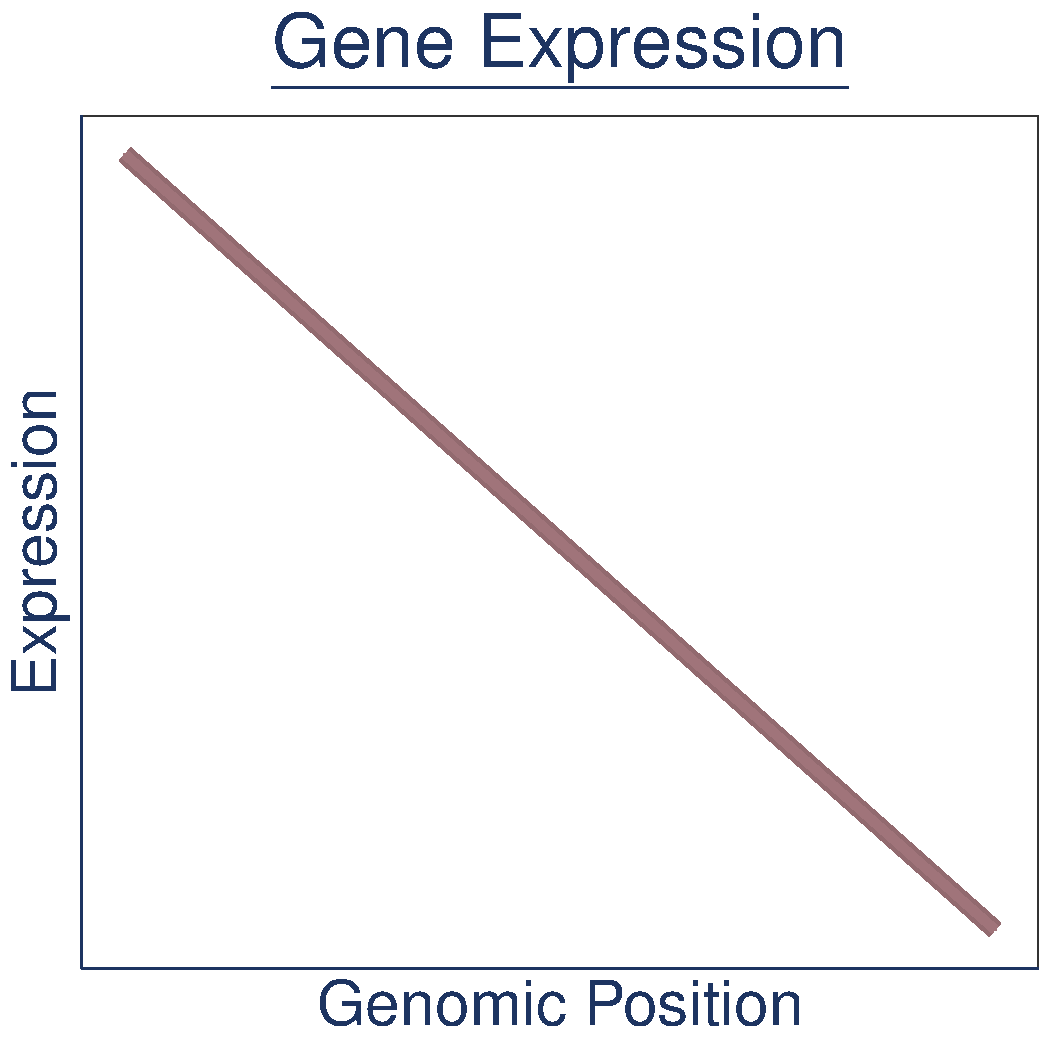
\includegraphics[width=0.34\textwidth]{C:/Users/Daniella/Documents/Sinorhizobium2015/LabMeetingPresentations/Spatial_genome_trends_graphs/exp_graph.pdf}
%%		\column{.5\textwidth}
%%		\centering
%%		\includegraphics[width=0.67\textwidth]{C:/Users/Daniella/Documents/Sinorhizobium2015/LabMeetingPresentations/Spatial_genome_trends_graphs/ess_graph.pdf}\\
%%		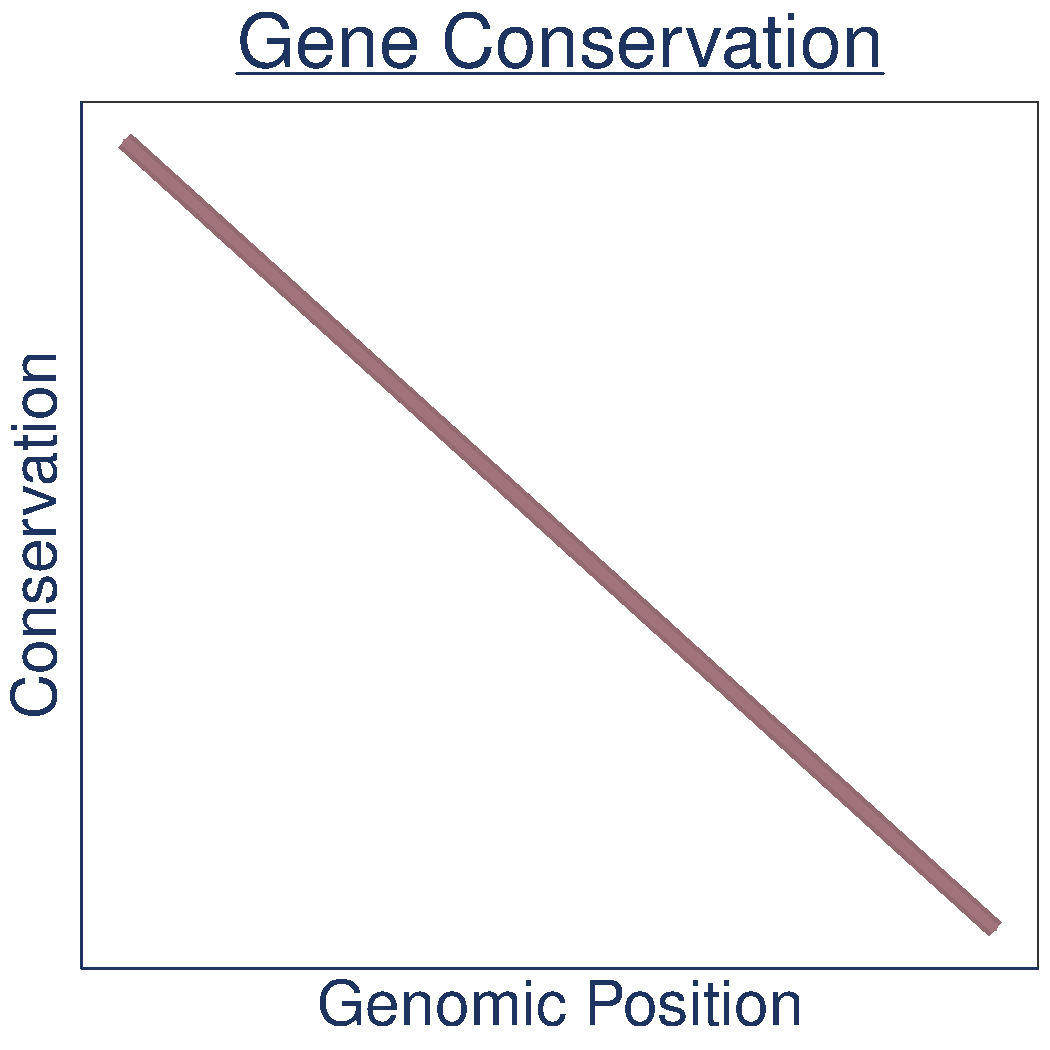
\includegraphics[width=0.67\textwidth]{C:/Users/Daniella/Documents/Sinorhizobium2015/LabMeetingPresentations/Spatial_genome_trends_graphs/cons_graph.pdf}
%%	\end{columns}
%	
%	\btVFill
%	\tiny \vspace{-\baselineskip}\color{berry}{Couturier et al. 2006, Cooper et al. 2010, Sharp et al. 2005, Morrow et al. 2012, Cooper and Rocha 2006, \\ Juurik et al. 2012, Hudson et al. 2002}
%	%		\sourceright{Couturier et al. 2006, Cooper et al. 2010, Sharp et al. 2005, Morrow et al. 2012, Cooper and Rocha 2006}
%	
%\end{frame}
%%%%%%%%%%%%%%%%%%%%%%%%%%%%%%%%%%%%%%%%%%%%%%%%%%%	
%\begin{frame}{Problem:}
%	\begin{center}
%		\LARGE
%		Limited number of genomes!
%	\end{center}
%\end{frame}	
%%%%%%%%%%%%%%%%%%%%%%%%%%%%%%%%%%%%%%%%%%%%%%%%%%%	
%\begin{frame}{Solution:}
%	\begin{center}
%		\LARGE
%		Add more genomes!
%	\end{center}
%\end{frame}	
%
%%%%%%%%%%%%%%%%%%%%%%%%%%%%%%%%%%%%%%%%%%%%%%%%%%%	
%\begin{frame}[t]{Complications}
%	\bi
%	\itm Genomic Structure
%	\itm Genome Reorganization
%	\ei
%\end{frame}	
%%%%%%%%%%%%%%%%%%%%%%%%%%%%%%%%%%%%%%%%%%%%%%%%%%%
%\begin{frame}[t]{Complications}
%	\bi
%	\itm Genomic Structure
%	\itm \light{Genome Reorganization}
%	\ei
%	\bigskip
%	\begin{columns}[t]
%		\column{0.30\textwidth}
%		\textbf{1) Circular}
%		\centering
%		\begin{tikzpicture}
%		%circle
%		\draw[thick] (4,0) circle (1cm);
%		%origin tick
%		\draw[thick] (4,0.8) -- (4,1.2);
%		\tikzstyle{none}=[draw = none, minimum width=2cm, minimum height=0.3cm, rounded corners]
%		\node[none] (first reservoir) at (4,-4) {\ecoli};
%		\tikzstyle{ntwo}=[draw = none, minimum width=2cm, minimum height=0.3cm, rounded corners]
%		\node[ntwo] (second reservoir) at (4,-4.5) {\bas};
%		\end{tikzpicture}
%		
%		\column{0.30\textwidth}
%		\textbf{2) Linear}
%		\centering
%		
%		\bigskip
%		\begin{tikzpicture}
%		%line
%		\draw[thick] (3.5,0) -- (6.5,0);
%		%origin tick
%		\draw[thick] (4.5,-.2) -- (4.5,.2);
%		\tikzstyle{none}=[draw = none, minimum width=2cm, minimum height=0.3cm, rounded corners]
%		\node[none] (first reservoir) at (5,-5.1) {\strep};
%		\end{tikzpicture}
%		
%		\column{0.4\textwidth}
%		\textbf{3) Multi-repliconic}
%		\centering
%		\begin{tikzpicture}
%		%chrom
%		\draw[thick] (0,0) circle (1cm) node {\tiny Chromosome};
%		%ori tick
%		\draw[thick] (0,0.8) -- (0,1.2);
%		%pSymA
%		\draw[thick] (0,-1.75) circle (0.5cm) node {\tiny \pa};
%		%ori tick
%		\draw[thick] (0,-1.1) -- (0,-1.4);
%		%pSymB
%		\draw[thick] (0,-3.25) circle (0.75cm) node {\tiny \pb};
%		%ori tick
%		\draw[thick] (0,-2.35) -- (0,-2.65);
%		\tikzstyle{none}=[draw = none, minimum width=2cm, minimum height=0.3cm, rounded corners]
%		\node[none] (first reservoir) at (0,-4.5) {\sm};
%		\end{tikzpicture}
%	\end{columns}
%\end{frame}
%%%%%%%%%%%%%%%%%%%%%%%%%%%%%%%%%%%%%%%%%%%%%%%%%%
%\begin{frame}[t]{Complications}
%	\bi
%	\itm \light{Genomic Structure}
%	\itm Genome Reorganization
%	\ei
%	\bigskip 
%	
%%	Rearrangements increase with an increased number of repeated sequences
%	
%	\bigskip
%	\begin{columns}
%		\column{0.5\textwidth}
%		\begin{centering}
%			\includegraphics[width=\textwidth]{C:/Users/Daniella/Documents/Sinorhizobium2015/Figs/Alignments/5completed_genomes_chroms.jpg}
%			
%			
%		\end{centering}
%		
%		\column{0.5\textwidth}
%		\begin{centering}
%			\includegraphics[width=\textwidth]{C:/Users/Daniella/Documents/Sinorhizobium2015/Figs/Alignments/12_sino_chroms_mauve_alignment_25Jun18.jpg}
%			
%		\end{centering}
%	\end{columns}
%%	\sourceextremeright{{\tiny \color{berry}{Rocha 2004, 2008}}}	
%\end{frame}
%%	\begin{frame}{Spatial Molecular Trends}
%%		Other Analysis:
%%		
%%		\bigskip
%%		No correlation between mutation rate and distance from the origin
%%		
%%		\bigskip
%%		But, mutation rates vary with position in \ecol and \salm
%%		
%%		\bigskip
%%%		\sourceright{Juurik et al. 2012, Hudson et al. 2002}
%%	\end{frame}	
%%%%%%%%%%%%%%%%%%%%%%%%%%%%%%%%%%%%%%%%%%%%%%%%%%%%	
%%\begin{frame}{Horizontal Gene Transfer and Selection in \s}
%%
%%HGT
%%\begin{itemize}
%%\item<itm@1-> Occurs almost exclusively on the plasmids, accounting for most of nucleotide diversity
%%\item<itm@1-> Strongest in areas involved in symbiosis with host plant
%%\item<itm@1-> May be geographical structuring
%%\item<itm@1-> Recent transfer followed by transfer sequences separating through recipient species
%%\end{itemize}
%
%%Selection
%%\begin{itemize}
%%\item<itm@1-> Symbiosis, survival and reproduction, nutrient acquisition, and stress tolerance
%%\item<itm@1-> Different selective forces on each strain
%%\item<itm@1-> Stronger purifying selection against non-synonymous mutations, HGT, and duplications
%%\end{itemize}
%
%%\bigskip
%% \btVFill
%
%%\small Epstein et al. 2014, Galardini et al. 2013, Galibert et al. 2001
%%\end{frame}
%%%%%%%%%%%%%%%%%%%%%%%%%%%%%%%%%%%%%%%%%%%%%%%%%%%
%%\begin{frame}{Opposing Trends}
%%	Point mutation rates vary with chromosome position but do not increase with distance from the origin
%%	
%%	\bigskip
%%	\begin{itemize}
%%		\item<itm@1-> \textit{Salmonella enterica}
%%		\item<itm@1-> Moved two lacZ alleles
%%		\item<itm@1-> Mutation rates not affected by neighbouring sequence		
%%	\end{itemize}
%%%	
%%	\small Hudson et al. 2002
%%	
%%\end{frame}
%%%%%%%%%%%%%%%%%%%%%%%%%%%%%%%%%%%%%%%%%%%%%%%%%%%
%%\begin{frame}{Why?}
%%       \begin{itemize}
%%       	\item<itm@1-> Recombination rate less regulated
%%       	\item<itm@1-> Core and dispensable genome placement
%%     %  	\item<itm@1-> Replicon placement
%%     %  	\itm Transposon insertion event
%%       	\itm Gene order
%%       	\itm Nucleotide composition
%%       \end{itemize} 
%%       %	\begin{center}
%%       %		\adjustbox{max width=\textwidth}{
%%       %		\begin{tabular}{l|c|c}
%%       %			\toprule
%%       %			\textbf{Authors} & \textbf{Species Name} & \textbf{Genomic Structure}\\
%%       %			\midrule
%%       %			Galardini et al. 2013 & \s (14 genomes) & 1 chromosome, 2 plasmids\\
%%       %			\midrule
%%       %			Morrow et al. 2012 & \bur (4 genomes) & 3 chromosomes\\
%%       %			\midrule
%%       %			Cooper et al. 2010 & \begin{tabular}{@{}r@{}}\bur (6 genomes) \\ \bor (4 genomes) \\ \vib (4 genomes) \\ \xan (5 genomes) %\end{tabular} & \begin{tabular}{@{}c@{}} 3 chromosomes \\ single circular chromosome \\ 2 chromosomes \\ single circular chromosome  %\end{tabular} \\
%%       %			\midrule
%%       %			Couturier et al. 2006 & 126 species of bacteria (only chromosome) & \begin{tabular}{@{}c@{}}only primary chromosome \\ for multi-repliconic bacteria\end{tabular} \\
%%       %			\midrule
%%       %			Flynn et al. 2010 & \sul (6 genomes) & single circular chromosome \\
%%       %			\midrule
%%       %			Sharp et al. 2005 & 80 species of bacteria (genomic) & \begin{tabular}{@{}c@{}}only primary chromosome \\ for multi-repliconic bacteria\end{tabular}  \\
%%       %			\bottomrule
%%       %		\end{tabular}
%%       %	}
%%       %	\end{center}%Sharp et al. 2005: 80 genomes from various bacteria, (single chromosome, one genome per strain)
%%       \btVFill
%%       {\tiny \color{berry}{Flynn et al. 2010, Couturier and Rocha 2006, Sharp et al. 2005, Gerdes et al. 2003, Mackiewicz et al. 2001, Mackiewicz et al. 1999, Karlin 2001}}
%%\end{frame}
%
%
%%%%%%%%%%%%%%%%%%%%%%%%%%%%%%%%%%%%%%%%%%%%%%%%%%%
%
%\begin{frame}{Research Objective}
%%	\begin{enumerate}
%%		\item How do various molecular trends change with genome position in bacteria?
%		
%		\textbf{How do various molecular trends change with genome position in bacteria?}
%		
%		\be
%		\item Substitutions
%		\item Gene Expression
%		\ee
%		
%%		\item \light{Determine the impact large and small scale inversions have on gene expression in bacteria.}
%%	\end{enumerate}
%	\bigskip
%	
%	
%	
%	\begin{itemize}
%		\item<itm@1-> Accounting for rearrangements and inversions
%		\bi
%		\itm Ancestral reconstruction
%		\itm Genome alignment
%		\ei
%		\itm Increasing the number of genomes
%		%\item<itm@1-> Looking at all regions of the genome (coding and non-coding)
%		%\item<itm@1-> Varying genomic structures
%		%\itm Ancestral state of substitutions and their genomic positions
%		%\item<itm@1-> Large number of genomes in each species
%		%\item<itm@1-> Hypothesize that substitution rates will increase when moving away from the origin of replication
%		%\item<itm@1-> Plasmids vs. Chromosome
%		%\begin{itemize}
%		%	\item<itm@1-> Chromosome $<$ Plasmid B $<$ Plasmid A
%		%\end{itemize}
%		
%	\end{itemize}
%	
%	
%	%      Do the trends vary between bacterial genomic structures, regions, and genomes?
%	%      
%	%     	\bigskip
%	%     	How selection impacts different bacteria
%\end{frame}
%%%%%%%%%%%%%%%%%%%%%%%%%%%%%%%%%%%%%%%%%%%%%%%%%%%
%\begin{frame}{Bacterial Genomes}
%	25 complete bacterial genomes:
%	\bi
%	\itm \ecoli (6 strains)
%	\itm \bas (7 strains)
%	\itm \strep (6 species)
%	\itm \sm (6 strains)
%	\ei
%\end{frame}
%%%%%%%%%%%%%%%%%%%%%%%%%%%%%%%%%%%%%%%%%%%%%%%%%%%
%\begin{frame}{Substitution Analysis}
%%	\centering{
%	\resizebox{0.9\textwidth}{!}{%
%	\tikzstyle{none}=[fill=pgreen, draw, minimum width=2cm, minimum height=0.5cm, rounded corners]
%	\tikzstyle{ntwo}=[fill=pgreen, draw, minimum width=2cm, minimum height=0.5cm, rounded corners]
%	\tikzstyle{nthree}=[fill=pgreen, draw, minimum width=2cm, minimum height=0.5cm, rounded corners]
%	\tikzstyle{nfour}=[fill=pgreen, draw, minimum width=2cm, minimum height=0.5cm, rounded corners]
%	\tikzstyle{nfive}=[fill=pgreen, draw, minimum width=2cm, minimum height=0.5cm, rounded corners]
%	\tikzstyle{nsix}=[fill=pgreen, draw, minimum width=2.5cm, minimum height=0.5cm, rounded corners]
%	\tikzstyle{nseven}=[fill=pgreen, draw, minimum width=2cm, minimum height=0.5cm, rounded corners]
%	\tikzstyle{neight}=[fill=pgreen, draw, minimum width=2cm, minimum height=0.5cm, rounded corners]
%	\tikzstyle{nnine}=[fill=pgreen, draw, minimum width=2cm, minimum height=0.5cm, rounded corners]
%	\tikzstyle{nten}=[fill=pgreen, draw, minimum width=2cm, minimum height=0.5cm, rounded corners]
%	\tikzstyle{nten}=[fill=pgreen, draw, minimum width=2cm, minimum height=0.5cm, rounded corners]
%	\tikzstyle{neleven}=[draw = none, minimum width=2cm, minimum height=0.5cm, rounded corners]
%	\tikzstyle{ntwelve}=[draw = none, minimum width=2cm, minimum height=0.5cm, rounded corners]
%	\begin{tikzpicture}
%	\footnotesize
%	\node[none] (first reservoir) at (0,0) {Genome Data};
%	\node[ntwo] (second reservoir) at (0,-1.06) {Whole Genome Alignment};
%	\node[nthree] (third reservoir) at (0,-2.13) {Phylogenetic Tree Construction};
%%	\node[nfour, align=center] (forth reservoir) at (0,-2.4) {Phylogenetic Tree Construction};
%	\node[nfive, align=center] (fifth reservoir) at (0,-3.19) {Ancestral Reconstruction};
%	\node[nsix, align=center] (sixth reservoir) at (-1.4,-4.25) {Nucleotide};
%	\node[nseven, align=center] (seventh reservoir) at (1.4,-4.25) {Genome Position};
%	\node[neight, align=center] (eighth reservoir) at (0,-5.31) {Logistic Regression};
%%	\node[nnine, align=center] (ninth reservoir) at (0,-5.6) {Removing Outliers and Gaps};
%%	\node[nten, align=center] (tenth reservoir) at (0,-6.4) {Logistic Regression};
%%	\node[neleven, align=left] (eleventh reservoir) at (9,-1.05) {\p \\ \begin{varwidth}{\linewidth}\begin{itemize}
%%		\itm \textbf{L}ocally \textbf{C}ollinear \textbf{B}locks (\textbf{LCBs})
%%		\end{itemize}\end{varwidth}};
%%	\node[ntwelve, align=left] (tvelveth reservoir) at (6,-4) {\includegraphics[width=.5\textwidth]{C:/Users/Daniella/Documents/Sinorhizobium2015/Papers/Substitutions_paper/Substitutions_paper/Figs/Bacillus_alignment_mauve.jpg}};
%	\draw[->] (first reservoir.south) -- (second reservoir.north);
%	\draw[->] (second reservoir.south) -- (third reservoir.north);
%	\draw[->] (third reservoir.south) -- (fifth reservoir.north);
%%	\draw[->] (forth reservoir.south) -- (fifth reservoir.north);
%	\draw[->] (fifth reservoir.south) -- (sixth reservoir.north);
%	\draw[->] (fifth reservoir.south) -- (seventh reservoir.north);
%	\draw[->] (sixth reservoir.south) -- ([xshift=-0.5cm]eighth reservoir.north);
%	\draw[->] (seventh reservoir.south) -- ([xshift=0.5cm]eighth reservoir.north);
%%	\draw[->] (eighth reservoir.south) -- (ninth reservoir.north);
%%	\draw[->] (ninth reservoir.south) -- (tenth reservoir.north);
%%	\draw[->] (second reservoir.east) -- (eleventh reservoir.west);
%	\end{tikzpicture}
%}%resize box
%%}%centering
%%	\sourceextremeright{{\tiny \color{berry}{Darling et al. 2010}}}
%\end{frame}
%%%%%%%%%%%%%%%%%%%%%%%%%%%%%%%%%%%%%%%%%%%%%%%%%%%
%
%\begin{frame}{Substitution Logistic Regression}
%	\begin{minipage}{\textwidth}
%		\begin{table}[h!]
%			\centering
%			\resizebox{\textwidth}{!}{%
%				\begin{tabular}{lccc}
%					\toprule
%					Bacteria and Replicon & \multicolumn{2}{c}{Slope} & Genome Structure\\
%					\cmidrule{2-3}
%					& Coding Sites & Non-Coding Sites & \\
%					\midrule
%					\ecol Chromosome & \ccbb-9.119\e{-8}*** & 7.022\e{-8}***  &  \color{berry}{\textbigcircle}\\
%					\bass Chromosome & \ccbb-1.273\e{-7}*** & \ccbb -9.861\e{8}*** &  \color{berry}{\textbigcircle}\\
%					\strep Chromosome & \ccbb -7.945\e{-9}*** & 3.637\e{-7}*** & \color{berry}{-----}\\
%					\smel Chromosome & \ccbb-1.550\e{-7}***& \ccbb-1.510\e{-7}* &  \color{berry}{\textbigcircle}  \color{db}{\APLcirc{}} \xspace \color{db}{\xspace \APLcirc{}}\\
%					\smel pSymA & \ccbb-1.156\e{-7}* & NS &  \color{db}{\textbigcircle}  \color{berry}{\APLcirc{}} \xspace \color{db}{\xspace \APLcirc{}}\\
%					\smel pSymB & 2.587\e{-7}*** & 8.591\e{-7}*** & \color{db}{\textbigcircle}  \color{db}{\xspace \APLcirc{}} \xspace \color{berry}{\APLcirc{}}\\
%					\bottomrule
%				\end{tabular}
%			}%resizebox
%			%	\caption{\label{tab:tabel2} Logistic regression analysis of the number of substitutions along the genome of the respective bacteria replicons. Grey coloured boxes indicate a negative logistic regression coefficient estimate. All results are statistically significant. Logistic regression was calculated after the origin of replication was moved to the beginning of the genome and all subsequent positions were scaled around the origin accounting for bidirectionality of replication.}
%		\end{table}
%		{\tiny Significance Codes: p $<$ 0.001 = `***', 0.001 $<$ 0.01 = `**', 0.01 $<$ 0.05 = `*', NS = Not Significant}
%		
%		\bigskip
%		\centering
%		Most bacteria have spatial substitution trends that were%
%		
%		{\large\textbf{not expected}!}%
%	\end{minipage}
%\end{frame}
%%%%%%%%%%%%%%%%%%%%%%%%%%%%%%%%%%%%%%%%%%%%%%%%%%%
%\begin{frame}{Decreasing Substitution Trend}
%	Number of substitutions decreases with increasing distance from the origin of replication
%	\bigskip
%	
%	\textbf{Near the Origin of Replication:}
%	\begin{columns}[T]
%		\begin{column}{0.5\textwidth}
%			\bi
%			\item<itm@1->  Transposon insertion $\uparrow$
%			\itm Potential genomic and pathogenecity islands $\uparrow$
%			\itm Multiple replication forks
%			\bi
%			
%			\itm Rearrangements and translocations
%			\ei
%			%			\item<itm@1->  Transposon insertion peaks at origin and is at minimum at terminus in \ecol
%			\ei
%		\end{column}
%		\begin{column}{0.35\textwidth}  %%<--- here
%			
%			\bi
%			\item[$\rightarrow$] Asymmetry in nucleotide composition
%			\item[$\rightarrow$] GC Content
%			\item[$\rightarrow$] Mutations
%			\ei
%		\end{column}
%	\end{columns}
%	\bigskip
%	
%	%
%	
%	%	\begin{itemize}
%	
%	%		\item<itm@1-> Potential genomic and pathogenecity islands near the origin of \ecol, \tub, and \hal
%	%		\item<itm@1-> Replication forks are sites for rearrangements and translocations
%	
%	
%	%	\end{itemize}
%	%			\textbf{Organelle Example:} Mitochondria have $\uparrow$ substitution rate in the control region
%	%			\bi
%	%			\itm High concentration of polymorphisms
%	%			\ei
%	\btVFill
%	\tiny \vspace{-\baselineskip}\color{berry}{Gerdes et al. 2003, Ikeda et al. 2003, Mackiewicz et al. 1999, Karlin 2001, Mira et al. 2010, \\ Pesole et al. 1999, Stoneking et al. 1991}
%	
%	%       \sourceright{Gerdes et al. 2003, Ikeda et al. 2003, Mackiewicz et al. 1999, Karlin 2001, Mira et al. 2010}
%\end{frame}
%%%%%%%%%%%%%%%%%%%%%%%%%%%%%%%%%%%%%%%%%%%%%%%%%%%
%
%\begin{frame}{Gene Expression Analysis}
%	\centering{
%		\resizebox{0.6\textwidth}{!}{%
%	\tikzstyle{none}=[fill=pgreen, draw, minimum width=2cm, minimum height=0.8cm, rounded corners]
%	\tikzstyle{ntwo}=[fill=pgreen, draw, minimum width=2cm, minimum height=0.8cm, rounded corners]
%	\tikzstyle{nthree}=[fill=pgreen, draw, minimum width=2cm, minimum height=0.8cm, rounded corners]
%	\tikzstyle{nfour}=[fill=pgreen, draw, minimum width=2cm, minimum height=0.8cm, rounded corners]
%	\tikzstyle{nfive}=[fill=pgreen, draw, minimum width=2cm, minimum height=0.8cm, rounded corners]
%	\tikzstyle{nsix}=[draw= none, minimum width=2cm, minimum height=0.8cm, rounded corners]
%	\tikzstyle{nseven}=[draw= none, minimum width=2cm, minimum height=0.8cm, rounded corners]
%	\begin{tikzpicture}
%	\footnotesize
%	\node[none] (first reservoir) at (0,0) {Raw Expression Data};
%	\node[ntwo] (second reservoir) at (0,-1.32) {Normalization};
%	\node[nthree] (third reservoir) at (0,-2.65) {Genome Position};
%	\node[nfour, align=center] (forth reservoir) at (0,-3.97) {Linear Regression};
%%	\node[nfive, align=center] (fifth reservoir) at (0,-3.2) {Linear Regression};
%%	\node[nsix, align=left] (sixth reservoir) at (10,-1) {\textbf{G}ene \textbf{E}xpression \textbf{O}mnibus (\textbf{GEO})\\
%%		\begin{varwidth}{\linewidth}\begin{itemize}
%%		\itm \ecol
%%		\itm \bass
%%		\itm \strep
%%		\itm \smel
%%		\itm Control Data
%%		\end{itemize}\end{varwidth} 
%%	};
%	\draw[->] (first reservoir.south) -- (second reservoir.north);
%	\draw[->] (second reservoir.south) -- (third reservoir.north);
%	\draw[->] (third reservoir.south) -- (forth reservoir.north);
%%%	\draw[->] (forth reservoir.south) -- (fifth reservoir.north);
%%	\draw[->] (first reservoir.east) -- (sixth reservoir.west);
%	\end{tikzpicture}
%}%resize box
%}%centering
%%	\sourceextremeright{{\tiny \color{berry}{Barrett et al. 2012}}}
%\end{frame}
%
%%%%%%%%%%%%%%%%%%%%%%%%%%%%%%%%%%%%%%%%%%%%%%%%%%%
%	
%	\begin{frame}{Gene Expression Linear Regression}
%		\begin{minipage}{\textwidth}
%			\begin{table}[h!]
%				\centering
%				\resizebox{\textwidth}{!}{%
%					\begin{tabular}{lccc}
%						\toprule
%						Bacteria and Replicon & Slope & P-value & Genome Structure\\
%						\midrule
%						\ccbb\ecol Chromosome & \ccbb-6.03\e{-5}  & \ccbb2.8\e{-6} & \ccbb \color{berry}{\textbigcircle}\\
%						\ccbb\bass Chromosome & \ccbb-9.7\e{-5} & \ccbb1.2\e{-6} & \ccbb \color{berry}{\textbigcircle} \\
%						\ccbb\strep Chromosome & \ccbb-1.17\e{-6} & \ccbb$<$2\e{-16} & \ccbb \color{berry}{-----}\\
%						\smel Chromosome & 3.97\e{-5} & NS & \color{berry}{\textbigcircle}  \color{db}{\APLcirc{}}  \xspace \color{db}{\xspace \APLcirc{}} \\
%						\smel pSymA & 1.39\e{-3} & 4.9\e{-8} & \color{db}{\textbigcircle}  \color{berry}{\APLcirc{}}  \xspace \color{db}{\xspace \APLcirc{}} \\
%						\smel pSymB & 1.46\e{-4} & NS & \color{db}{\textbigcircle}  \color{db}{\APLcirc{}}    \xspace \color{berry}{\xspace \APLcirc{}} \\
%						\bottomrule
%					\end{tabular}
%					
%				}%resizebox
%				%	\caption{\label{tab:lr_exp} Linear regression analysis of the median counts per million expression data along the genome of the respective bacteria replicons. Grey coloured boxes indicate statistically significant results at the 0.5 significance level. Linear regression was calculated after the origin of replication was moved to the beginning of the genome and all subsequent positions were scaled around the origin accounting for bidirectionality of replication.}
%			\end{table}
%			{\tiny NS = Not Significant}
%			
%			\bigskip
%			\centering
%			Most bacteria have spatial gene expression trends that%
%			
%			{\large\textbf{matched expectations}!}%
%		\end{minipage}
%	\end{frame}
%%%%%%%%%%%%%%%%%%%%%%%%%%%%%%%%%%%%%%%%%%%%%%%%%%% 
%
%
%\begin{frame}{Summary of Results}
%	\begin{table}[h]
%		\centering
%		\resizebox{\textwidth}{!}{%
%			\begin{tabular}{l*{4}{C}}
%				\toprule
%				Bacteria and Replicon & \multicolumn{2}{c}{Number of Substitutions} & Gene Expression & Genome Structure\\
%				\cmidrule{2-3}
%				& Coding & Non-Coding & & \\
%				\midrule
%				\ecol Chromosome & \ccb $\downarrow$ & \cc $\uparrow$ & \ccb $\downarrow$ & \color{berry}{\textbigcircle}\\
%				\bass Chromosome & \ccb $\downarrow$ & \ccb $\downarrow$ & \ccb $\downarrow$ & \color{berry}{\textbigcircle}\\
%				\strep Chromosome & \ccb $\downarrow$ & \cc $\uparrow$ & \ccb $\downarrow$ & \color{berry}{-----}\\
%				\smel Chromosome &  \ccb $\downarrow$& \ccb $\downarrow$  & NS & \color{berry}{\textbigcircle}  \color{db}{\APLcirc{}} \xspace \color{db}{\xspace \APLcirc{}}\\
%				\smel pSymA & \ccb $\downarrow$ & NS & \cc $\uparrow$ & \color{db}{\textbigcircle}  \color{berry}{\APLcirc{}} \xspace \color{db}{\xspace \APLcirc{}}\\
%				\smel pSymB & \cc $\uparrow$ & \cc $\uparrow$ & NS  & \color{db}{\textbigcircle}  \color{db}{\xspace \APLcirc{}} \xspace \color{berry}{\APLcirc{}}\\
%				\bottomrule
%			\end{tabular}
%		}%resizebox
%		%	\caption{\label{tab:tabel2} Logistic regression analysis of the number of substitutions along the genome of the respective bacteria replicons. Grey coloured boxes indicate a negative logistic regression coefficient estimate. All results are statistically significant. Logistic regression was calculated after the origin of replication was moved to the beginning of the genome and all subsequent positions were scaled around the origin accounting for bidirectionality of replication.}
%	\end{table}
%	\tiny NS = Not Significant 
%\end{frame}
%%%%%%%%%%%%%%%%%%%%%%%%%%%%%%%%%%%%%%%%%%%%%%%%%%%
%\begin{frame}{Conclusions}
%	\begin{columns}[t]
%		\column{.5\textwidth}
%		\centering
%		\textbf{Previous Studies:} 
%		
%		\bigskip
%		\includegraphics[width=0.65\textwidth]{C:/Users/Daniella/Documents/Sinorhizobium2015/LabMeetingPresentations/Spatial_genome_trends_graphs/mut_graph.pdf}\\
%		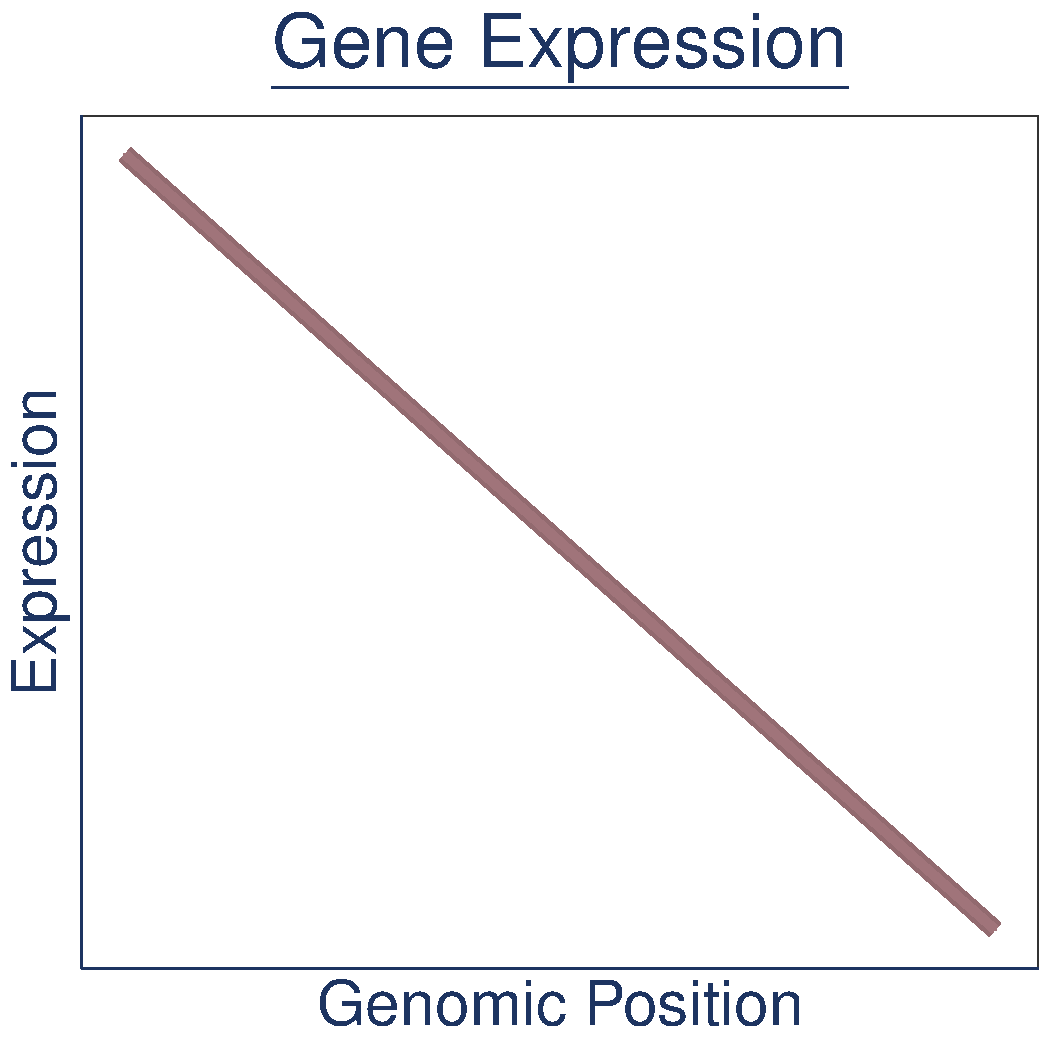
\includegraphics[width=0.65\textwidth]{C:/Users/Daniella/Documents/Sinorhizobium2015/LabMeetingPresentations/Spatial_genome_trends_graphs/exp_results_graph.pdf}
%		\column{.5\textwidth}
%		\centering
%		\textbf{This Study:}
%		
%		\bigskip
%		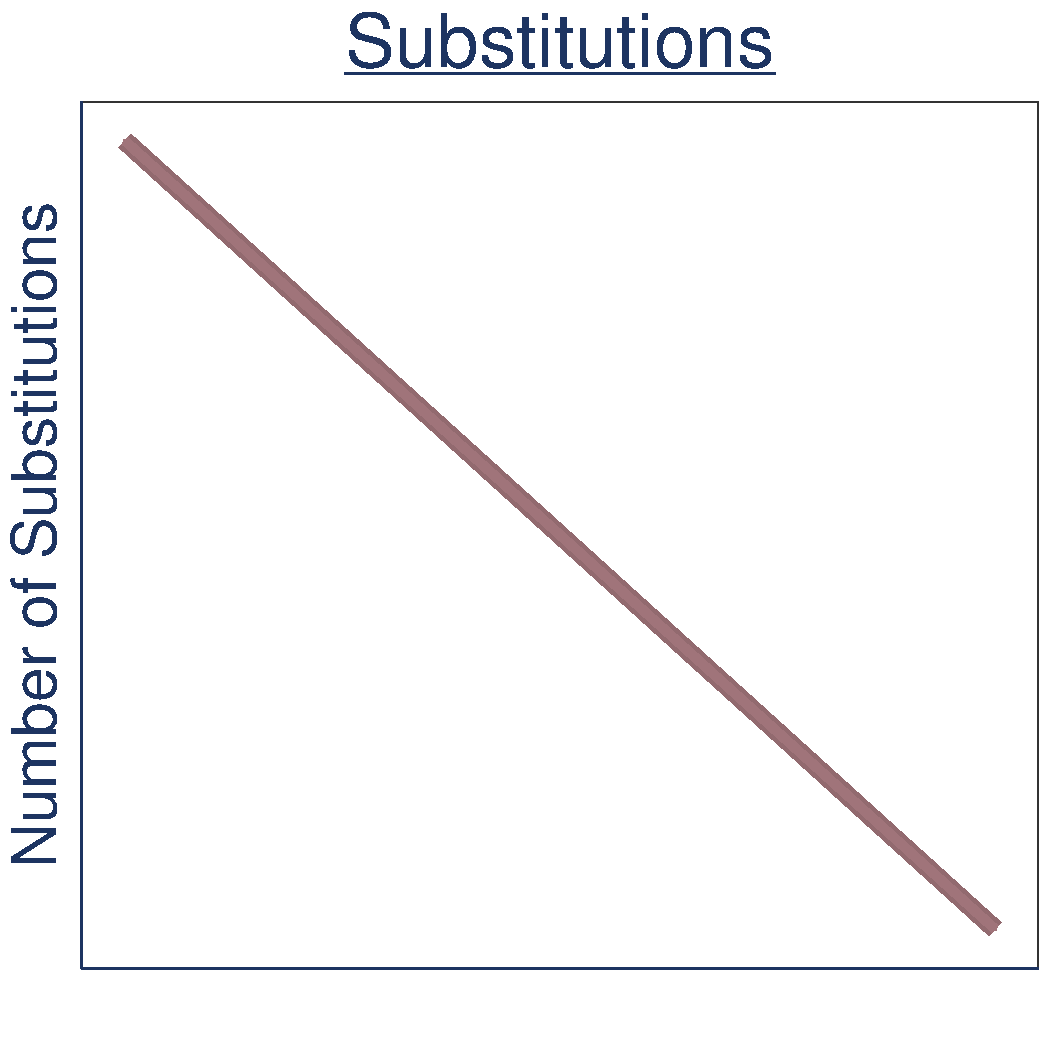
\includegraphics[width=0.65\textwidth]{C:/Users/Daniella/Documents/Sinorhizobium2015/LabMeetingPresentations/Spatial_genome_trends_graphs/sub_results_graph.pdf}\\
%		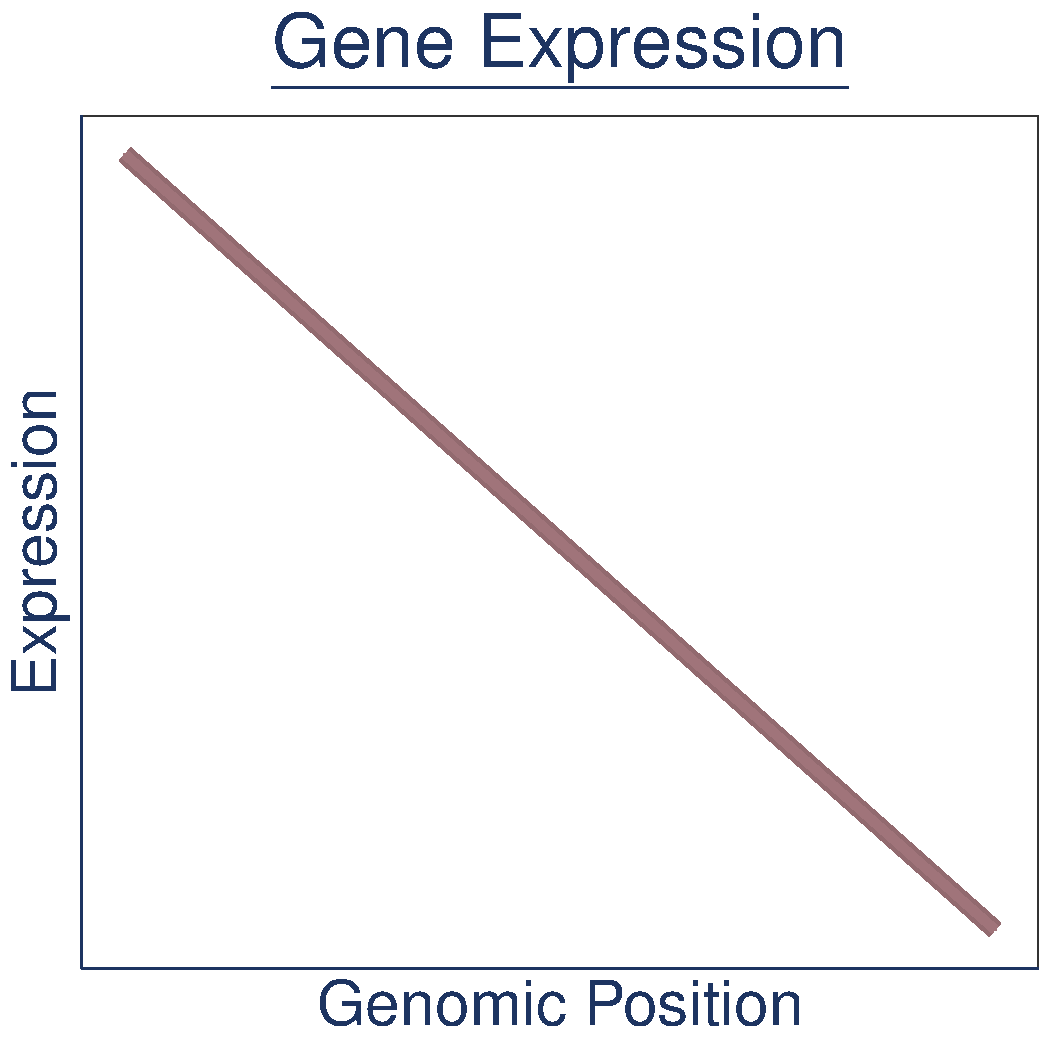
\includegraphics[width=0.65\textwidth]{C:/Users/Daniella/Documents/Sinorhizobium2015/LabMeetingPresentations/Spatial_genome_trends_graphs/exp_results_graph.pdf}
%	\end{columns}
%\end{frame}
%%%%%%%%%%%%%%%%%%%%%%%%%%%%%%%%%%%%%%%%%%%%%%%%%%%
%%\begin{frame}{Summary}
%%	
%%	Provide an updated review and analysis of spatial substitution trends in \ecol, \bass, \strep and \smel.
%%	\bi
%%%	\itm Protein Function
%%	\itm Gene Expression
%%%	\itm GC Content
%%%	\itm Total Number of Genes 
%%	\ei
%%	Increase the general knowledge of bacterial genome organization.
%%	
%%\end{frame}
%%%%%%%%%%%%%%%%%%%%%%%%%%%%%%%%%%%%%%%%%%%%%%%%%%%
%\begin{frame}{Future Research}
%\LARGE
%	\begin{enumerate}
%	\item Selection on coding sequences
%	\bi
%	\itm per gene dN/dS
%	\itm per genome dN/dS
%	\ei
%	\item Impact of inversions on gene expression
%	\end{enumerate}
%\end{frame}
%
%%%%%%%%%%%%%%%%%%%%%%%%%%%%%%%%%%%%%%%%%%%%%%%%%%%
%\begin{frame}{Thanks To:}
%	\begin{columns}[t]
%		\column{0.5\textwidth}
%		\bi
%		\itm Dr. G. Brian Golding
%		\itm Dr. Ben Evans
%		\itm Dr. Marie Elliot
%		\ei
%		
%		
%		
%		\column{0.5\textwidth}
%		\bi
%		\itm The Golding Lab
%		\itm The Evans Lab
%		\ei
%	\end{columns}
%	
%	\bigskip
%	\btVFill
%	\includegraphics[width=.3\textwidth,center]{C:/Users/Daniella/Documents/Sinorhizobium2015/Conferences/ISMB_Chicago_2018/mcm-col.jpg}
%		\bigskip
%	
%	
%		\btVFill\includegraphics[scale=0.4]{C:/Users/Daniella/Documents/Sinorhizobium2015/Conferences/ISMB_Chicago_2018/NSERC_FIP_RGB.jpg}
%	\bigskip
%\end{frame}
%%%%%%%%%%%%%%%%%%%%%%%%%%%%%%%%%%%%%%%%%%%%%%%%%%%
%\begin{frame}{}
%	\centering
%	\Huge Supplementary Information
%\end{frame}
%%%%%%%%%%%%%%%%%%%%%%%%%%%%%%%%%%%%%%%%%%%%%%%%%%%
%\begin{frame}{Supplementary Information}
%	\begin{table}[h]
%		\centering
%		\resizebox{\textwidth}{!}{%
%			\begin{tabular}{lrrrrr}
%				\toprule
%				Bacteria and Replicon & Average Replicon Length & \# of Coding Sites & \# of Non-Coding Sites & \# of Subs Coding & \# of Subs Non-Coding\\
%				\midrule
%				\ecol Chromosome & 5082529 & 5203089 & 191748 & 169620 & 9534 \\ % 4048616/4641652 & 
%				\bass Chromosome & 4077077 & 2074653 & 102906 & 171351 & 6187\\ %3692179/4215606
%				\strep Chromosome & 8497577 & 1996354 & 18584 & 246447 & 2808\\ % 7628849/8667507
%				\smel Chromosome & 3426881 & 1931139 & 199425 & 5141 & 842\\ % 3130925/3654135
%				\smel pSymA & 1455940 & 419223 & 34213 & 7647 & 943\\ % 1128615/1354226 & 225611/1354226
%				\smel pSymB & 1664597 & 552816 & 22098 & 10032 & 645\\ % 1493048/1683333
%				\bottomrule
%			\end{tabular}
%			
%		}%resizebox
%%		\caption{\label{tab:cod_non_cod_proportions} Total proportion of coding and non-coding sites in each replicon and the percentage of those sites that have a substitution (multiple substitutions at one site are counted as two substitutions).}
%	\end{table}
%	
%\end{frame}
%	%%%%%%%%%%%%%%%%%%%%%%%%%%%%%%%%%%%%%%%%%%%%%%%%%%	
%	\begin{frame}{\ecol}
%		
%		\begin{figure}
%			\begin{center}
%				\includegraphics[scale=0.46]{C:/Users/Daniella/Documents/Sinorhizobium2015/Figs/Sub_graphs_cod_non_cod_7Feb19/ecoli_chrom_cod_non_cod_sub_histogram_bidirectionality_colour_25Apr19.pdf}
%			\end{center}
%		\end{figure}
%	\end{frame}
%	%%%%%%%%%%%%%%%%%%%%%%%%%%%%%%%%%%%%%%%%%%%%%%%%%%
%	
%	\begin{frame}{\bass}
%		
%		\begin{figure}
%			\begin{center}
%				\includegraphics[scale=0.46]{C:/Users/Daniella/Documents/Sinorhizobium2015/Figs/Sub_graphs_cod_non_cod_7Feb19/bass_chrom_cod_non_cod_sub_histogram_bidirectionality_colour_25Apr19.pdf}
%			\end{center}
%		\end{figure}
%	\end{frame}
%	%%%%%%%%%%%%%%%%%%%%%%%%%%%%%%%%%%%%%%%%%%%%%%%%%%
%	
%	\begin{frame}{\strep}
%		\begin{figure}
%			\begin{center}
%				\includegraphics[scale=0.46]{C:/Users/Daniella/Documents/Sinorhizobium2015/Figs/Sub_graphs_cod_non_cod_7Feb19/strep_chrom_cod_non_cod_sub_histogram_bidirectionality_colour_26Apr19.pdf}
%			\end{center}
%		\end{figure}
%	\end{frame}
%	%%%%%%%%%%%%%%%%%%%%%%%%%%%%%%%%%%%%%%%%%%%%%%%%%%
%	
%	\begin{frame}{\smel Chromosome}
%		%\begin{columns}[t]
%		%    \column{0.5\textwidth}
%		%    \scriptsize{Plasmid A: Codon Position 2}\includegraphics[scale=0.07]{Lato3.pdf}
%		\begin{figure}
%			\begin{center}
%				\includegraphics[scale=0.46]{C:/Users/Daniella/Documents/Sinorhizobium2015/Figs/Sub_graphs_cod_non_cod_7Feb19/sinoC_chrom_cod_non_cod_sub_histogram_bidirectionality_colour_25Apr19.pdf}
%			\end{center}
%		\end{figure}
%		
%		%    \column{0.5\textwidth}
%		%    \scriptsize{Palsmid A}\includegraphics[scale=0.07]{Lato2.pdf}
%		%    \begin{figure}
%		% \begin{center}
%		%           \includegraphics[scale=0.22]{ex_rate_position2.pdf} 
%		%            \end{center}
%		%            \end{figure}
%		
%		%\end{columns}
%	\end{frame}
%	%%%%%%%%%%%%%%%%%%%%%%%%%%%%%%%%%%%%%%%%%%%%%%%%%%
%	
%	\begin{frame}{\smel pSymA}
%		
%		\begin{figure}
%			\begin{center}
%				\includegraphics[scale=0.46]{C:/Users/Daniella/Documents/Sinorhizobium2015/Figs/Sub_graphs_cod_non_cod_7Feb19/pSymA_chrom_cod_non_cod_sub_histogram_bidirectionality_colour_25Apr19.pdf}
%			\end{center}
%		\end{figure}
%	\end{frame}
%	%%%%%%%%%%%%%%%%%%%%%%%%%%%%%%%%%%%%%%%%%%%%%%%%%%
%	
%	\begin{frame}{\smel pSymB}
%		
%		\begin{figure}
%			\begin{center}
%				
%				\includegraphics[scale=0.46]{C:/Users/Daniella/Documents/Sinorhizobium2015/Figs/Sub_graphs_cod_non_cod_7Feb19/pSymB_chrom_cod_non_cod_sub_histogram_bidirectionality_colour_25Apr19.pdf}
%			\end{center}
%		\end{figure}
%	\end{frame}
%	%%%%%%%%%%%%%%%%%%%%%%%%%%%%%%%%%%%%%%%%%%%%%%%%%%	
%	\begin{frame}{Supplementary Information}
%		\begin{figure}[H]
%			\begin{center}
%				\includegraphics[scale=0.46]{C:/Users/Daniella/Documents/Sinorhizobium2015/Gene_Expression_8Dec17/Gene_Expression/Graphs/ecoli_chrom_sub_exp_histogram_bidirectionality_colour_13Mar19.pdf}
%				
%			\end{center}
%		\end{figure}
%	\end{frame}
%		%%%%%%%%%%%%%%%%%%%%%%%%%%%%%%%%%%%%%%%%%%%%%%%%%%	
%		\begin{frame}{Supplementary Information}
%			\begin{figure}[H]
%				\begin{center}
%					\includegraphics[scale=0.46]{C:/Users/Daniella/Documents/Sinorhizobium2015/Gene_Expression_8Dec17/Gene_Expression/Graphs/bass_chrom_sub_exp_histogram_bidirectionality_colour_4Mar19.pdf}
%					
%				\end{center}
%			\end{figure}
%		\end{frame}
%		
%				%%%%%%%%%%%%%%%%%%%%%%%%%%%%%%%%%%%%%%%%%%%%%%%%%%	
%				\begin{frame}{Supplementary Information}
%					\begin{figure}[H]
%						\begin{center}
%						\includegraphics[scale=0.46]{C:/Users/Daniella/Documents/Sinorhizobium2015/Gene_Expression_8Dec17/Gene_Expression/Graphs/strep_chrom_sub_exp_histogram_bidirectionality_colour_4Mar19.pdf}
%						
%						\end{center}
%					\end{figure}
%				\end{frame}
%%%%%%%%%%%%%%%%%%%%%%%%%%%%%%%%%%%%%%%%%%%%%%%%%%%	
%				\begin{frame}{Supplementary Information}
%					\begin{figure}[H]
%						\begin{center}
%							\includegraphics[scale=0.46]{C:/Users/Daniella/Documents/Sinorhizobium2015/Gene_Expression_8Dec17/Gene_Expression/Graphs/smel_chrom_sub_exp_histogram_bidirectionality_colour_4Mar19.pdf}
%							
%							
%						\end{center}
%					\end{figure}
%				\end{frame}
%%%%%%%%%%%%%%%%%%%%%%%%%%%%%%%%%%%%%%%%%%%%%%%%%%%	
%\begin{frame}{Supplementary Information}
%	\begin{figure}[H]
%		\begin{center}
%		\includegraphics[scale=0.46]{C:/Users/Daniella/Documents/Sinorhizobium2015/Gene_Expression_8Dec17/Gene_Expression/Graphs/pSymA_sub_exp_histogram_bidirectionality_colour_4Mar19.pdf}
%		
%			
%		\end{center}
%	\end{figure}
%\end{frame}	
%%%%%%%%%%%%%%%%%%%%%%%%%%%%%%%%%%%%%%%%%%%%%%%%%%%	
%\begin{frame}{Supplementary Information}
%	\begin{figure}[H]
%		\begin{center}
%		\includegraphics[scale=0.46]{C:/Users/Daniella/Documents/Sinorhizobium2015/Gene_Expression_8Dec17/Gene_Expression/Graphs/pSymB_sub_exp_histogram_bidirectionality_colour_4Mar19.pdf}
%		
%		
%		\end{center}
%	\end{figure}
%\end{frame}					
%	%%%%%%%%%%%%%%%%%%%%%%%%%%%%%%%%%%%%%%%%%%%%%%%%%%	
%	\begin{frame}{Supplementary Information}
%		\begin{figure}[H]
%			\begin{center}
%				\includegraphics[scale=0.137]{C:/Users/Daniella/Documents/Sinorhizobium2015/Papers/Substitutions_paper/Substitutions_paper/Figs/ecoli_chrom_superseq_all_blocks_branchlengths_rooted_outtree_21Aug17.pdf}
%			\end{center}
%		\end{figure}
%	\end{frame}
%	%%%%%%%%%%%%%%%%%%%%%%%%%%%%%%%%%%%%%%%%%%%%%%%%%%
%	
%	\begin{frame}{Supplementary Information}
%		\begin{figure}[H]
%			\begin{center}
%				\includegraphics[scale=0.135]{C:/Users/Daniella/Documents/Sinorhizobium2015/Papers/Substitutions_paper/Substitutions_paper/Figs/bacillus_chrom_superseq_all_blocks_branchlengths_rooted_outtree_21Aug17.pdf}
%			\end{center}
%		\end{figure}
%	\end{frame}
%	%%%%%%%%%%%%%%%%%%%%%%%%%%%%%%%%%%%%%%%%%%%%%%%%%%
%	
%	\begin{frame}{Supplementary Information}
%		\begin{figure}[H]
%			\begin{center}
%				\includegraphics[scale=0.137]{C:/Users/Daniella/Documents/Sinorhizobium2015/Papers/Substitutions_paper/Substitutions_paper/Figs/strep_chrom_superseq_all_blocks_branchlengths_rooted_outtree_21Aug17.pdf}
%			\end{center}
%		\end{figure}
%	\end{frame}
%	%%%%%%%%%%%%%%%%%%%%%%%%%%%%%%%%%%%%%%%%%%%%%%%%%%
%	
%	\begin{frame}{Supplementary Information}
%		\begin{figure}[H]
%			\begin{center}
%				
%				\includegraphics[scale=0.135]{C:/Users/Daniella/Documents/Sinorhizobium2015/Papers/Substitutions_paper/Substitutions_paper/Figs/chrom_all_blocks_branchlengths_rooted_outtree_21Aug17.pdf}
%			\end{center}
%		\end{figure}
%	\end{frame}
%	\begin{frame}{Supplementary Information}
%		\begin{figure}[H]
%			\begin{center}
%				\includegraphics[scale=0.137]{C:/Users/Daniella/Documents/Sinorhizobium2015/Papers/Substitutions_paper/Substitutions_paper/Figs/pSymA_all_blocks_branchlengths_rooted_outtree_21Aug17.pdf}
%			\end{center}
%		\end{figure}
%	\end{frame}
%	\begin{frame}{Supplementary Information}
%		\begin{figure}[H]
%			\begin{center}
%				\includegraphics[scale=0.135]{C:/Users/Daniella/Documents/Sinorhizobium2015/Papers/Substitutions_paper/Substitutions_paper/Figs/pSymB_all_blocks_branchlengths_rooted_outtree_21Aug17.pdf}
%			\end{center}
%		\end{figure}
%	\end{frame}
%
%	%%%%%%%%%%%%%%%%%%%%%%%%%%%%%%%%%%%%%%%%%
%\begin{frame}{Supplementary Information}
%	\centering
%	\resizebox{\textwidth}{!}{
%		\begin{tabular}{lcc}
%			\toprule
%			Bacteria & Origin of Replication & Terminus of Replication \\
%			\midrule
%			\ecol & 3925744 & 1678398 \\
%			\bass & 1 & 1942542 \\
%			\strep & 3419363 & 1 \& 9054831\\
%			\smel Chromosome & 1 & 1735626 \\
%			\smel pSymA & 1350001 & 672888 \\
%			\smel pSymB & 55090 & 896756\\
%			\bottomrule
%		\end{tabular}
%		
%	}
%\end{frame}
%%%%%%%%%%%%%%%%%%%%%%%%%%%%%%%%%%%%%%%%%%%%%%%%%%%
%
%
%%\begin{frame}{Supplementary Information}
%%	\centering
%%	\resizebox{\textwidth}{!}{%
%%		\begin{tabular}{lr}
%%			\toprule
%%			Bacteria and Replicon & Average Number of Substitutions per bp \\
%%			\midrule
%%			\ecol Chromosome & 1.81\e{-4}\\
%%			\bass Chromosome & 7.73\e{-4}\\
%%			\strep Chromosome & 7.84\e{-4}\\
%%			\smel Chromosome & 2.42\e{-5}\\
%%			\smel pSymA & 1.58\e{-4}\\
%%			\smel pSymB & 5.63\e{-4}\\
%%			\bottomrule
%%		\end{tabular}
%%	}%resizebox
%%	
%%\end{frame}
%%
%%%%%%%%%%%%%%%%%%%%%%%%%%%%%%%%%%%%%%%%%%%%%%%%%%%
%\begin{frame}{Supplementary Information}
%	
%	\begin{table}[]
%		\centering
%		\resizebox{\textwidth}{!}{%
%			\begin{tabular}{lcccccc}
%				\toprule
%				Origin Location & \ecol Chromosome &\bass Chromosome & \strep Chromosome & \smel Chromosome &\smel pSymA & \smel pSymB\\
%				\midrule
%				Moved 100kb Left & -1.445\e{-7}*** & 4.374\e{-9}* &  6.909\e{-9}*** &  -1.316\e{-6}*** & -1.058\e{-6}*** & -4.313\e{-8}*\\
%				Moved 90kb Left & -1.544\e{-7}*** & -1.036\e{-7}*** & 5.677\e{-9}*** & -1.32\e{-6}*** & -1.246\e{-6}*** & 1.37\e{-8}\\
%				Moved 80kb Left& -1.65\e{-7}*** & -1.072\e{-7}*** & 8.11\e{-9}*** & -1.338\e{-6}*** & -1.398\e{-6}*** & 4.28\e{-8}*\\
%				Moved 70kb Left& -1.667\e{-7}*** & -1.102\e{-7}*** & 6.716\e{-9}*** & -1.363\e{-6}*** & -1.405\e{-6}*** & 8.93\e{-8}***\\
%				Moved 60kb Left& -1.64\e{-7}*** & -1.19\e{-7}*** & 8.7\e{-9}*** & -1.324\e{-6}*** & -1.394\e{-6}*** & 1.43\e{-7}***\\
%				Moved 50kb Left& -1.446\e{-7}*** & -1.211\e{-7}*** & 1.045\e{-8}*** & -1.36\e{-6}*** & -1.403\e{-6}*** & 1.36\e{-7}***\\
%				Moved 40kb Left& -1.4\e{-7}*** & -1.299\e{-7}*** & 1.214\e{-8}*** & -1.255\e{-6}*** & -1.422\e{-6}*** & 1.543\e{-7}***\\
%				Moved 30kb Left& -1.498\e{-7}*** & -1.292\e{-7}*** & 1.24\e{-8}*** & -1.26\e{-6}*** & -1.392\e{-6}*** & 1.63\e{-7}***\\
%				Moved 20kb Left& -1.51\e{-7}*** & -1.1\e{-7}*** & 1.395\e{-8}*** & -1.525\e{-6}*** & -1.412\e{-6}*** & 1.603\e{-7}***\\
%				Moved 10kb Left& -1.262\e{-7}*** & -2.602\e{-9} & 1.563\e{-8}*** &  -1.599\e{-6}*** &  -9.499\e{-7}*** & 2.973\e{-7}*** \\
%				Moved 10kb Right& -1.305\e{-7}*** & -2.045\e{-8}*** & 1.578\e{-8}*** & 1.614\e{-6}*** & -1.026\e{-6}*** & 1.208\e{-7}*** \\
%				Moved 20kb Right& -1.454\e{-7}*** & -1.006\e{-7}*** & 1.903\e{-8}*** & -1.634\e{-6}*** & -1.475\e{-6}*** & 1.649\e{-7}***\\
%				Moved 30kb Right& -1.548\e{-7}*** & -8.596\e{-8}*** & 2.046\e{-8}*** & -1.698\e{-6}*** & -1.417\e{-6}*** & 1.526\e{-7}***\\
%				Moved 40kb Right& -1.632\e{-7}*** & -8.378\e{-8}*** & 2.125\e{-8}*** & -1.719\e{-6}*** & -1.367\e{-6}*** & 1.589\e{-7}***\\
%				Moved 50kb Right& -1.856\e{-7}*** & -7.879\e{-8}*** & 1.957\e{-8}*** & -1.735\e{-6}*** & -1.277\e{-6}*** & 1.654\e{-7}***\\
%				Moved 60kb Right& -1.91\e{-7}*** & -6.98\e{-8}*** & 1.974\e{-8}*** & -1.788\e{-6}*** & -1.169\e{-6}*** & 1.645\e{-7}***\\
%				Moved 70kb Right& -1.892\e{-7}*** & -6.634\e{-8}*** & 1.934\e{-8}*** & -1.854\e{-6}*** & -1.059\e{-6}*** & 1.843\e{-7}***\\
%				Moved 80kb Right& -1.879\e{-7}** & -5.814\e{-8}*** & 2.313\e{-8}*** & -1.891\e{-6}*** & -9.07\e{-7}*** & 1.90\e{-7}***\\
%				Moved 90kb Right& -1.862\e{-7}*** & -4.314\e{-8}*** & 2.304\e{-8}*** & -1.865\e{-6}*** & -7.171\e{-7}*** & 2.415\e{-7}***\\
%				Moved 100kb Right& -1.799\e{-7}*** & -2.597\e{-8}*** &  1.945\e{-8}*** &  -1.525\e{-6}*** & -6.572\e{-7}*** & 3.095\e{-7}***\\
%				\bottomrule
%			\end{tabular}
%			
%		}%resizebox
%		%	\caption{\label{tab:tabel2} Logistic regression analysis of the number of substitutions along the genome of the respective bacteria replicons. All results are marked with significance codes as followed: $<$ 0.001 = `***', 0.001 $<$ 0.01 = `**', 0.01 $<$ 0.05 = `*', 0.05 $<$ 0.1 = `.', $>$ 0.1 = ` '. Logistic regression was calculated after the origin of replication was moved to the beginning of the genome and all subsequent positions were scaled around the origin accounting for bidirectionality of replication.}
%	\end{table}
%	\tiny{All results are marked with significance codes as followed: $<$ 0.001 = `***', 0.001 $<$ 0.01 = `**', 0.01 $<$ 0.05 = `*', 0.05 $<$ 0.1 = `.', $>$ 0.1 = ` '}
%	
%	%	\btVFill
%	\bigskip
%	\centering
%	\normalsize
%	Moving the origin of replication \textbf{does not} alter the spatial substitution results
%	
%\end{frame}
%
%
%	%%%%%%%%%%%%%%%%%%%%%%%%%%%%%%%%%%%%%%%%%%%%%%%%%%
\end{document}
